\documentclass[conference]{IEEEtran}
\usepackage[utf8]{inputenc}
\usepackage{amsmath,amssymb}
\usepackage{graphicx}
\usepackage{booktabs}
\usepackage{hyperref}
\usepackage{xcolor}
\usepackage{subcaption}
\usepackage{multirow}
\usepackage{array}
\usepackage{float}

\graphicspath{{../app/AI/figures/}{../Designs/}}

\title{Multi-Corruption Image Restoration and Style-Conditioned\\Face-to-Sketch Generation: A Generative AI System}
\author{\IEEEauthorblockN{Muhammad Umair}
\IEEEauthorblockA{Generative AI — Assignment 1\\
GitHub: \url{https://github.com/UmairisHuman}}}

\begin{document}
\maketitle

% ============================================================================
\begin{abstract}
This report presents four generative AI systems integrated into a single browser-based application: (1)~a universal multi-corruption denoising autoencoder, (2)~a hard-routed specialist restoration system with corruption classification, (3)~a jointly trained soft mixture-of-experts restoration model, and (4)~a style-conditioned face-to-sketch generator using a conditional GAN. All models are trained with PyTorch, optimized via Optuna, tracked with Weights~\&~Biases, exported to ONNX, and deployed through a React + FastAPI application running in Docker containers. The universal autoencoder achieves 24.72~dB PSNR on corrupted images, the hard-routed system reaches 24.86~dB with 99.88\% routing accuracy, the soft MoE improves to 25.59~dB through learned weighted blending, and the conditional GAN produces style-controlled sketches with an FID of 33.29.
\end{abstract}

% ============================================================================
\section{Introduction}

Image restoration seeks to recover clean images from degraded inputs corrupted by noise, blur, or occlusion. Traditional approaches train separate models per corruption type, but practical systems encounter mixed or unknown degradations. This work investigates three progressively sophisticated restoration architectures—universal, hard-routed, and soft mixture-of-experts—and additionally explores paired image-to-image translation through face-to-sketch synthesis.

All four tasks use the same application infrastructure: a React frontend communicates with a FastAPI backend that performs inference using ONNX Runtime. The system is containerized with Docker Compose for reproducible single-command deployment.

% ============================================================================
\section{Related Work}

\textbf{Denoising Autoencoders.} Vincent et al.~\cite{vincent2008} demonstrated that autoencoders trained to reconstruct clean inputs from corrupted versions learn robust representations. The combination of L1 reconstruction loss with the Structural Similarity Index (SSIM) loss~\cite{wang2004ssim} has become standard for perceptual image restoration.

\textbf{Mixture of Experts.} Shazeer et al.~\cite{shazeer2017} introduced sparsely-gated MoE layers for language models. In vision, routing mechanisms enable specialized sub-networks to handle distinct input conditions, with soft routing providing differentiable expert blending.

\textbf{Conditional GANs.} Isola et al.~\cite{isola2017} demonstrated paired image-to-image translation with U-Net generators and PatchGAN discriminators. Style conditioning via learned embeddings follows Dumoulin et al.~\cite{dumoulin2017}, who showed that per-style affine parameters in instance normalization capture artistic styles.

% ============================================================================
\section{Dataset Preparation}

\subsection{Oxford-IIIT Pet Dataset (Tasks 1--3)}

The Oxford-IIIT Pet Dataset contains images of 37 cat and dog breeds. All images were converted to RGB and resized to $128 \times 128$ pixels. The official training/validation set was split into 80\% training and 20\% validation using random seed 42. The official test set was reserved for final evaluation.

\subsubsection{Corruption Pipeline}

For each training image, one of four conditions is sampled with equal probability:
\begin{itemize}
    \item \textbf{Clean}: no corruption applied.
    \item \textbf{Salt-and-pepper noise}: pixel replacement probability sampled uniformly from $[0.02, 0.15]$.
    \item \textbf{Gaussian blur}: kernel size from $\{3, 5, 7\}$, $\sigma \sim U(0.5, 2.5)$.
    \item \textbf{Rectangular occlusion}: 1--3 black rectangles covering 10--35\% of the image area.
\end{itemize}

Training corruptions are applied dynamically at runtime. Validation and test corruptions use deterministic manifests with fixed seeds. For the test set, each corruption has three severity levels:

\begin{table}[h]
\centering
\caption{Test Set Corruption Severity Levels}
\label{tab:severity}
\begin{tabular}{llll}
\toprule
Corruption & Low & Medium & High \\
\midrule
Salt-and-pepper & $p=0.03$ & $p=0.08$ & $p=0.15$ \\
Gaussian blur & $(3, 0.7)$ & $(5, 1.5)$ & $(7, 2.5)$ \\
Occlusion & 10\%, 1 rect & 20\%, 2 rects & 35\%, 3 rects \\
\bottomrule
\end{tabular}
\end{table}

\subsection{FS2K Dataset (Task 4)}

The FS2K Facial Sketch Synthesis Dataset contains 2,104 paired photographs and sketches in three style categories. The official training portion was further split: 85\% training (899 pairs), 15\% validation (159 pairs), stratified by style (seed 42). The official test set (1,046 pairs) was reserved for evaluation. All images were resized to $128 \times 128$.

% ============================================================================
\section{Task 1: Universal Multi-Corruption Denoising Autoencoder}

\subsection{Architecture}

The universal DAE uses a convolutional encoder-decoder architecture with a compressed spatial latent representation. The encoder progressively reduces spatial dimensions through strided convolutions while increasing channel depth. A $1 \times 1$ convolutional bottleneck compresses the representation to the latent space, followed by dropout regularization.

The decoder mirrors the encoder using transposed convolutions. Two bottlenecked skip connections (channels reduced to 4 via $1 \times 1$ convolutions) connect the deepest encoder levels to corresponding decoder levels. These limited skips preserve fine spatial detail while maintaining a genuine bottleneck—zeroing the latent representation drops PSNR by 5.63~dB, confirming the bottleneck carries meaningful information.

\textbf{Architecture summary:} Encoder channels: 48-96-192-384, latent: $16 \times 8 \times 8 = 1024$ (compression ratio 8:1), 2 bottlenecked skip connections (4 channels each), 9.29M parameters.

\subsection{Loss Function}

The model is trained using a weighted combination of L1 and SSIM losses:
\begin{equation}
    \mathcal{L}_{\text{UDAE}} = \alpha \cdot \mathcal{L}_{\text{L1}}(x, \hat{x}) + (1 - \alpha) \cdot (1 - \text{SSIM}(x, \hat{x}))
\end{equation}

The SSIM computation uses an $11 \times 11$ Gaussian window with $\sigma = 1.5$, matching the Wang et al.\ formulation.

\subsection{Hyperparameter Optimization}

Optuna was used to search the following space (32+ trials completed):

\begin{table}[h]
\centering
\caption{Task 1 Optuna Search Space and Best Configuration}
\label{tab:t1optuna}
\begin{tabular}{lll}
\toprule
Parameter & Search Range & Best \\
\midrule
Learning rate & $[10^{-4}, 3 \times 10^{-3}]$ (log) & $7.7 \times 10^{-4}$ \\
Batch size & $\{16, 32, 64\}$ & 16 \\
Base channels & $\{32, 48, 64\}$ & 48 \\
Latent channels & $\{8, 16, 32, 64\}$ & 16 \\
Skip levels & $\{0, 1, 2\}$ & 2 \\
Skip channels & $\{2, 4, 8\}$ & 4 \\
Dropout & $[0.0, 0.3]$ & 0.071 \\
$\alpha$ (loss weight) & $[0.5, 0.95]$ & 0.520 \\
\bottomrule
\end{tabular}
\end{table}

\begin{figure}[h]
    \centering
    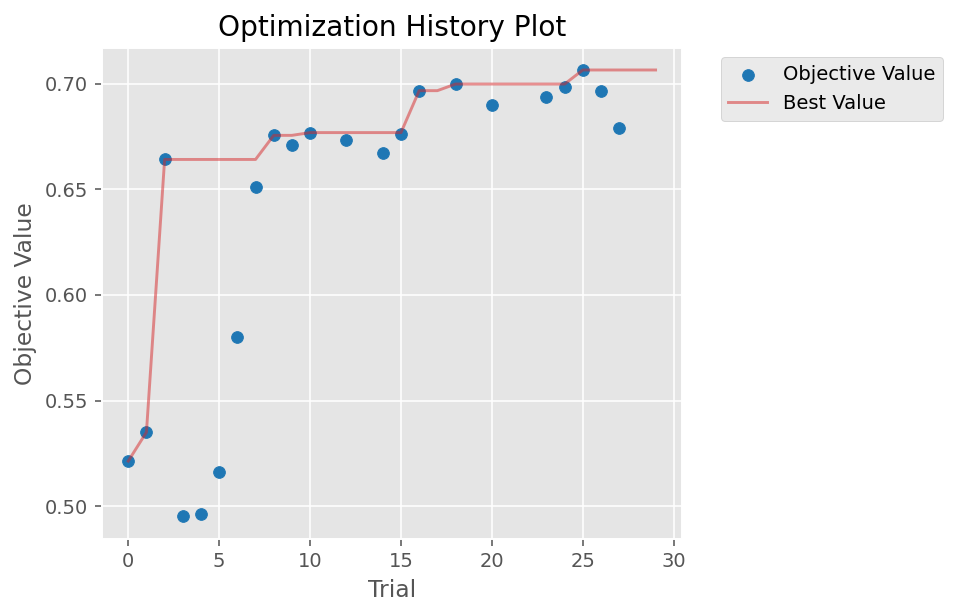
\includegraphics[width=\columnwidth]{task1/optuna_history.png}
    \caption{Task 1 Optuna optimization history.}
    \label{fig:t1optuna}
\end{figure}

\begin{figure}[h]
    \centering
    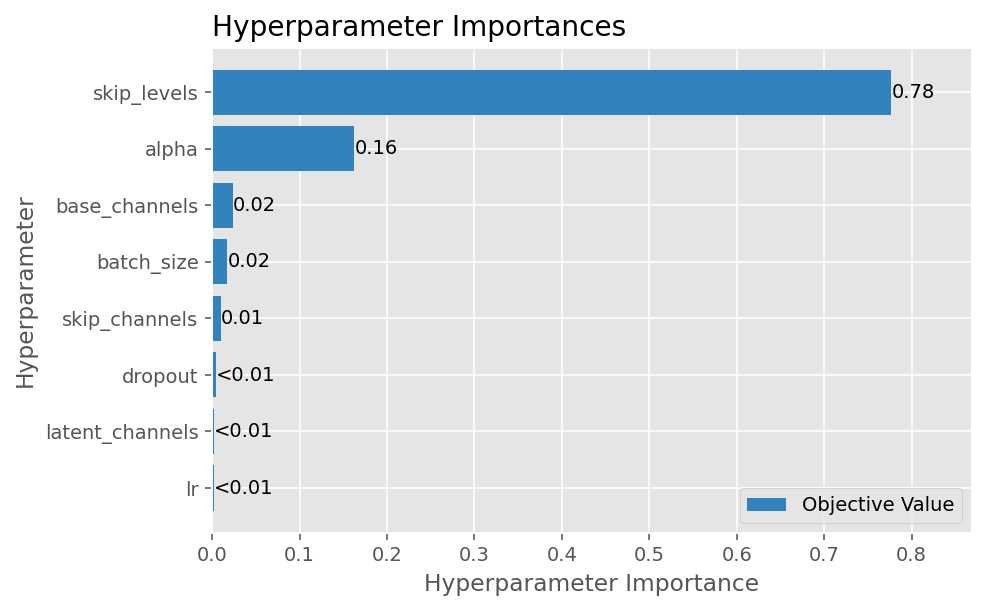
\includegraphics[width=\columnwidth]{task1/optuna_importance.png}
    \caption{Task 1 hyperparameter importance analysis.}
    \label{fig:t1importance}
\end{figure}

The near-equal weighting of L1 and SSIM ($\alpha \approx 0.52$) was selected by Optuna, differing from the suggested initial value of 0.8 and demonstrating the importance of the SSIM component.

\subsection{Results}

Training ran for 71 epochs (best validation score). The model was evaluated on the deterministic test set with results broken down by corruption type and severity.

\begin{table}[h]
\centering
\caption{Task 1 — Test Results by Corruption Type}
\label{tab:t1results}
\begin{tabular}{lcccc}
\toprule
Type & PSNR in & PSNR out & SSIM out & $\Delta$PSNR \\
\midrule
Clean & — & 26.78 & 0.897 & — \\
Salt-pepper & 16.38 & 26.73 & 0.891 & +10.35 \\
Gaussian blur & 27.82 & 25.67 & 0.845 & $-$2.15 \\
Occlusion & 13.56 & 21.76 & 0.779 & +8.20 \\
\midrule
All corrupted & 19.26 & 24.72 & 0.838 & +5.47 \\
\bottomrule
\end{tabular}
\end{table}

\begin{table}[h]
\centering
\caption{Task 1 — Test Results by Severity Level}
\label{tab:t1severity}
\begin{tabular}{llccc}
\toprule
Type & Severity & PSNR out & SSIM out & $\Delta$PSNR \\
\midrule
Salt-pepper & Low & 26.82 & 0.896 & +6.69 \\
Salt-pepper & Medium & 26.78 & 0.893 & +10.91 \\
Salt-pepper & High & 26.59 & 0.884 & +13.45 \\
\midrule
Gaussian blur & Low & 26.85 & 0.896 & $-$5.49 \\
Gaussian blur & Medium & 26.15 & 0.875 & $-$0.62 \\
Gaussian blur & High & 24.00 & 0.765 & $-$0.35 \\
\midrule
Occlusion & Low & 23.61 & 0.842 & +6.95 \\
Occlusion & Medium & 21.85 & 0.789 & +8.56 \\
Occlusion & High & 19.82 & 0.705 & +9.09 \\
\bottomrule
\end{tabular}
\end{table}

\begin{figure}[h]
    \centering
    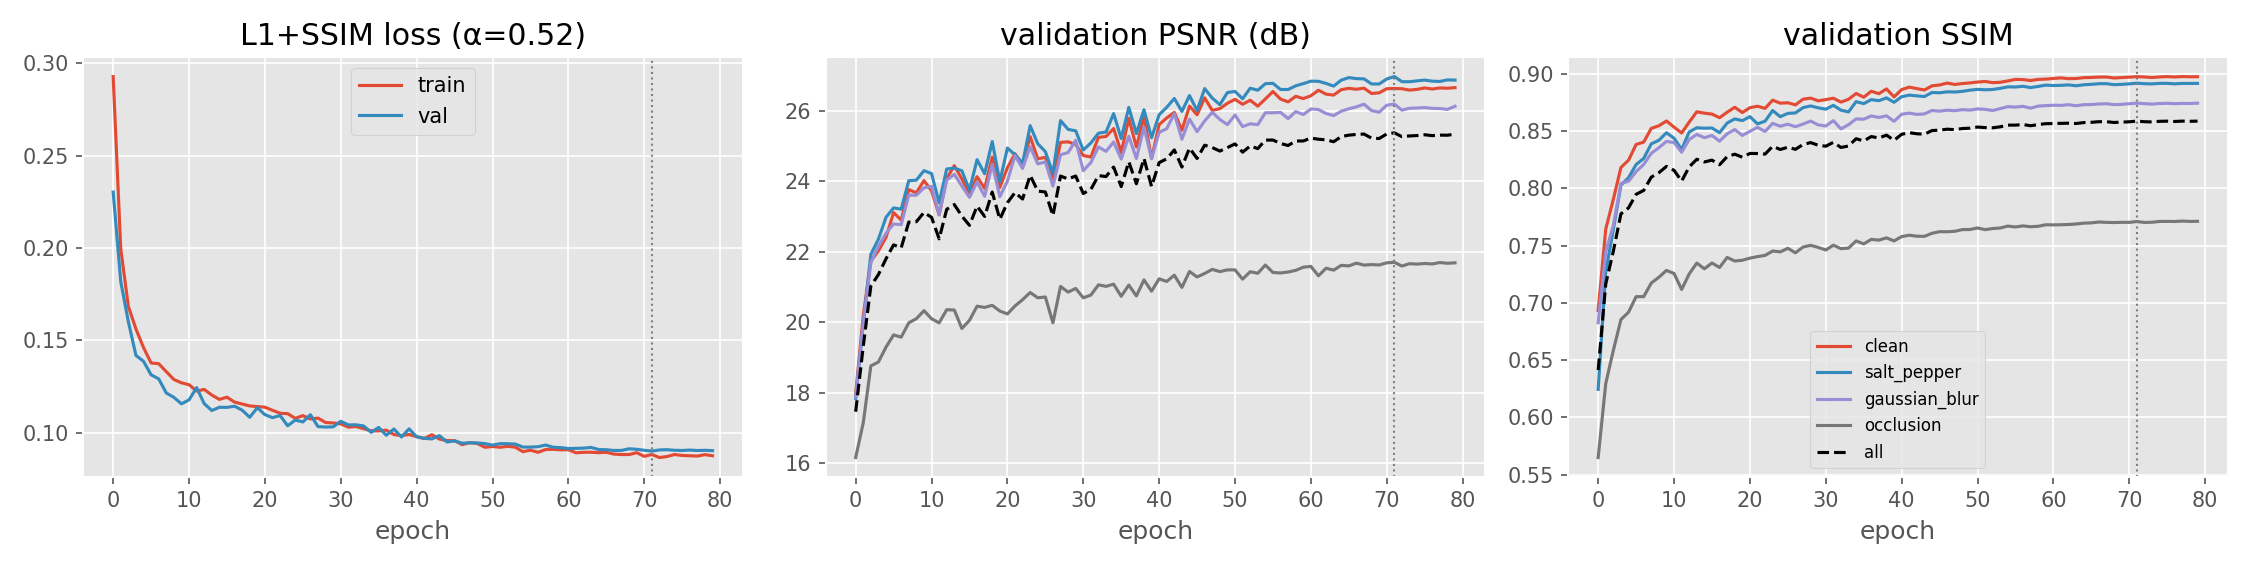
\includegraphics[width=\columnwidth]{task1/training_curves.png}
    \caption{Task 1 training and validation curves.}
    \label{fig:t1curves}
\end{figure}

\begin{figure}[h]
    \centering
    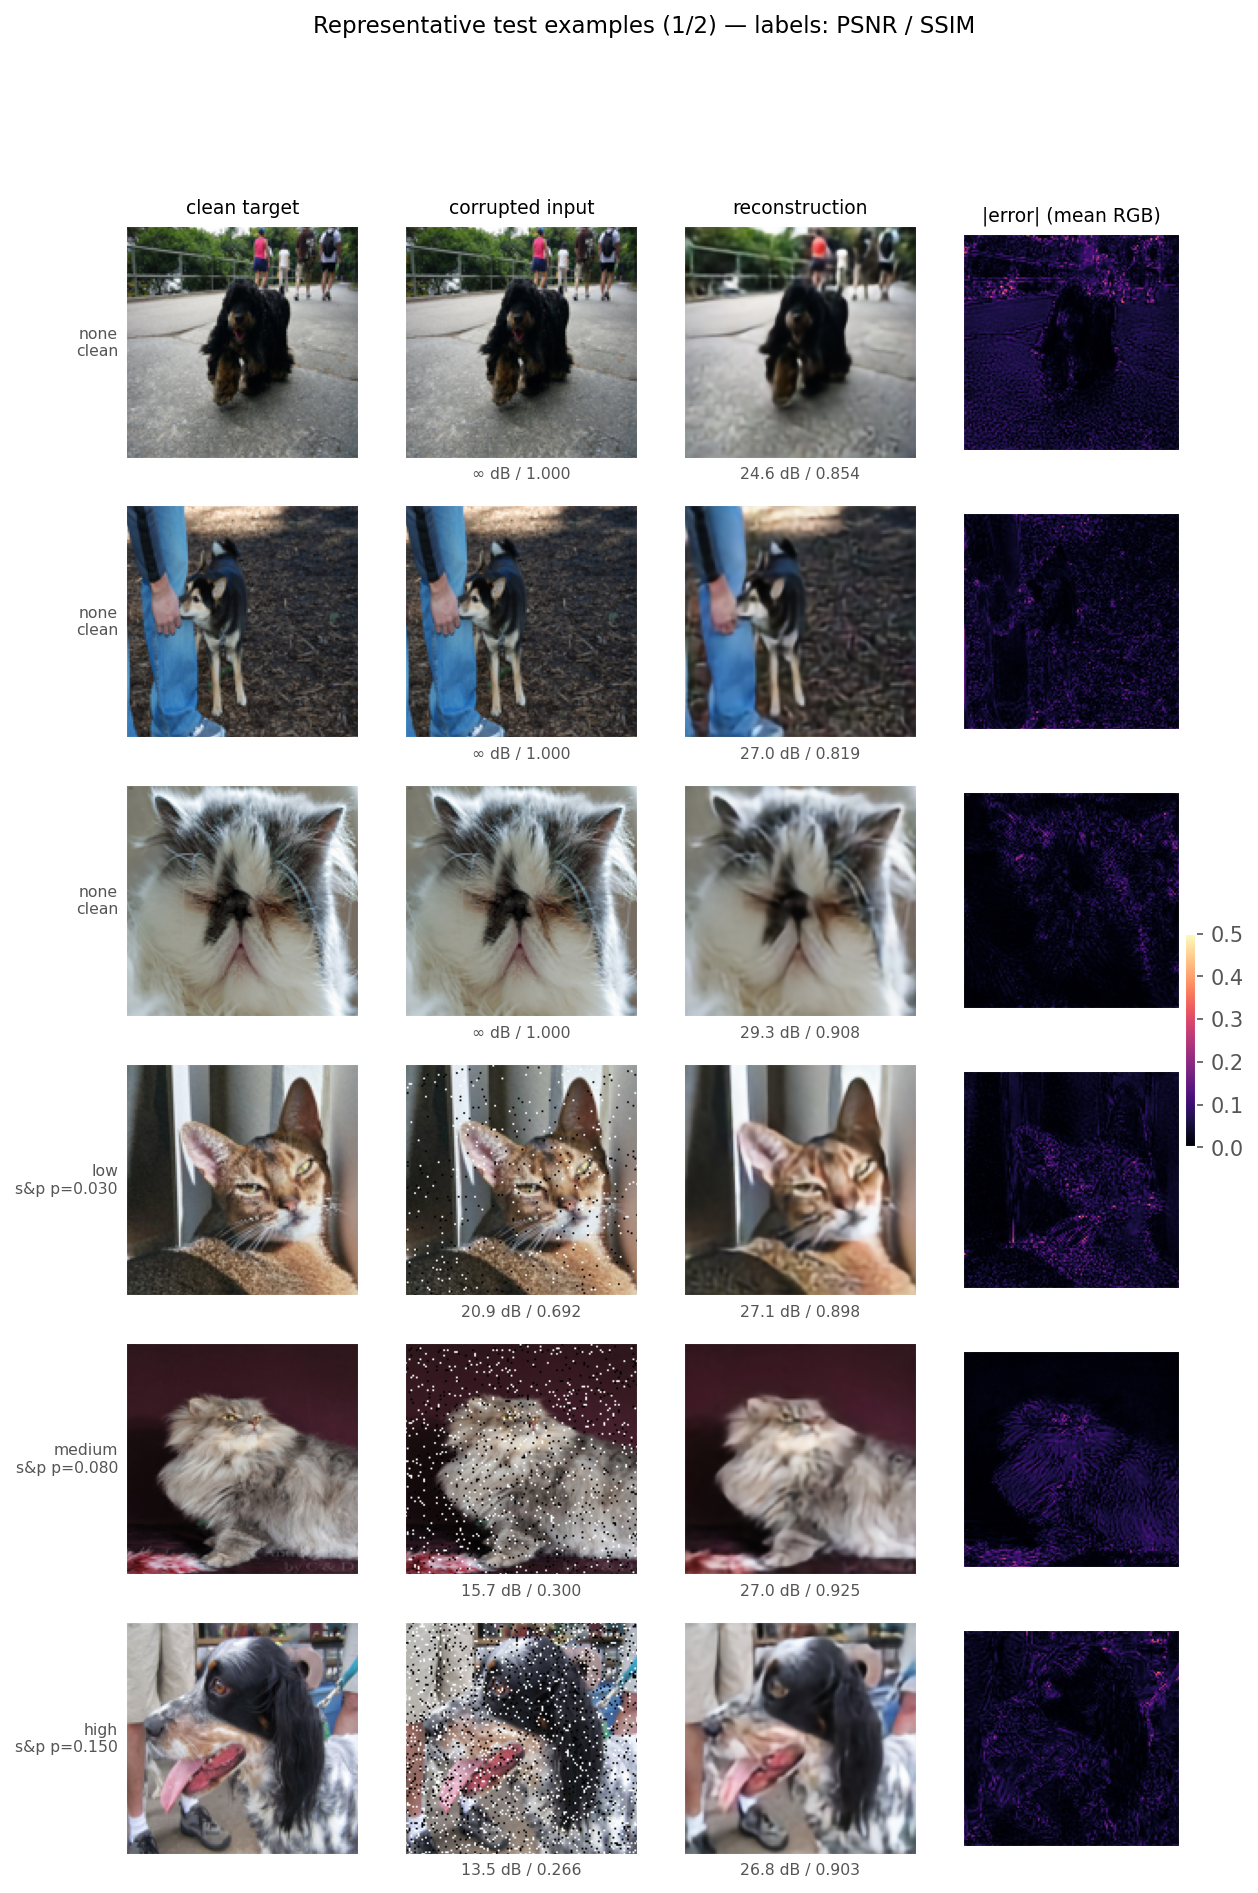
\includegraphics[width=\columnwidth]{task1/test_representative_1.png}
    \caption{Task 1 representative restoration results: clean target, corrupted input, restored output, and absolute error map.}
    \label{fig:t1examples}
\end{figure}

\begin{figure}[h]
    \centering
    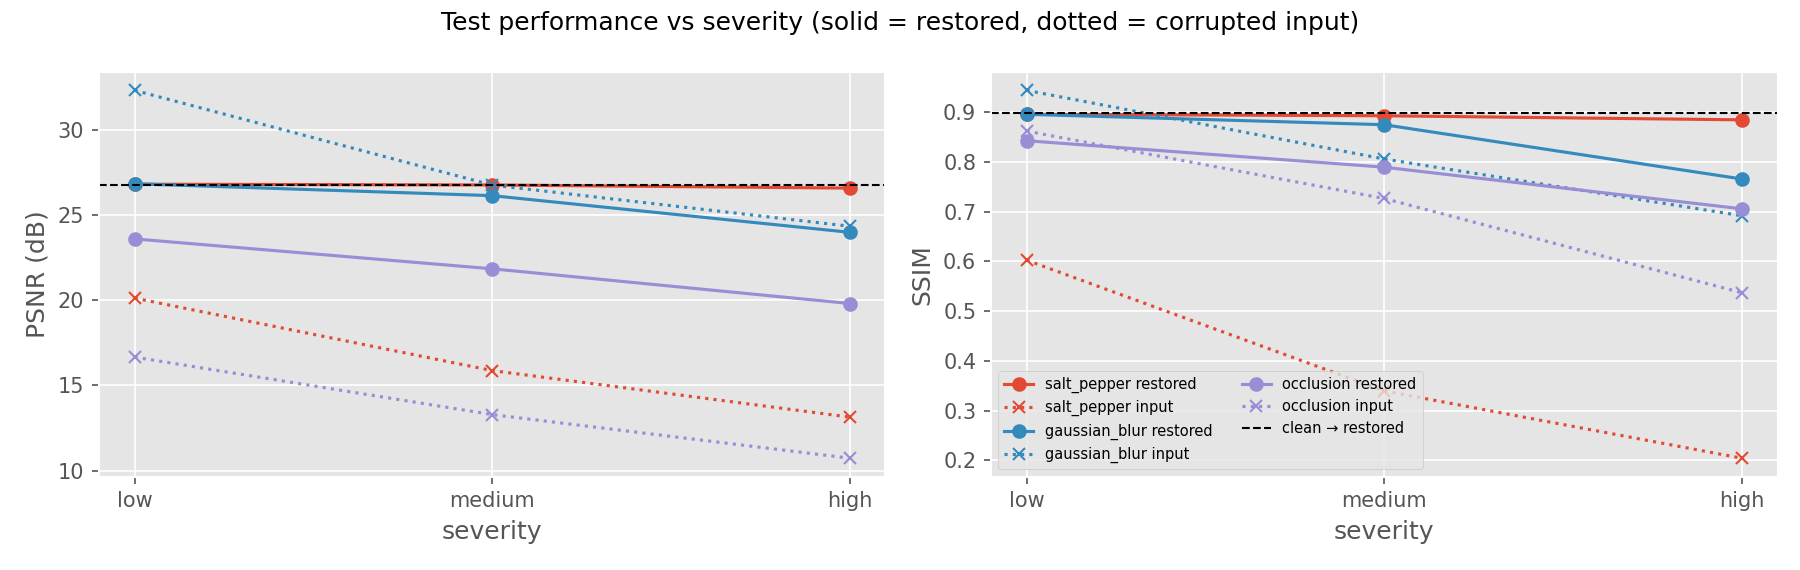
\includegraphics[width=\columnwidth]{task1/test_severity_curves.png}
    \caption{Task 1 PSNR and SSIM across corruption severity levels.}
    \label{fig:t1severity_curves}
\end{figure}

\textbf{Analysis.} Salt-and-pepper restoration is highly effective across all severities, with consistent output quality regardless of noise level. Gaussian blur produces a slight PSNR decrease at low severity because the blurred input already has high PSNR (low-frequency content retains pixel averages), but the model improves perceptual sharpness (SSIM increases). Occlusion restoration degrades gracefully with coverage: at 35\% coverage the model still achieves 19.82~dB.

\begin{figure}[h]
    \centering
    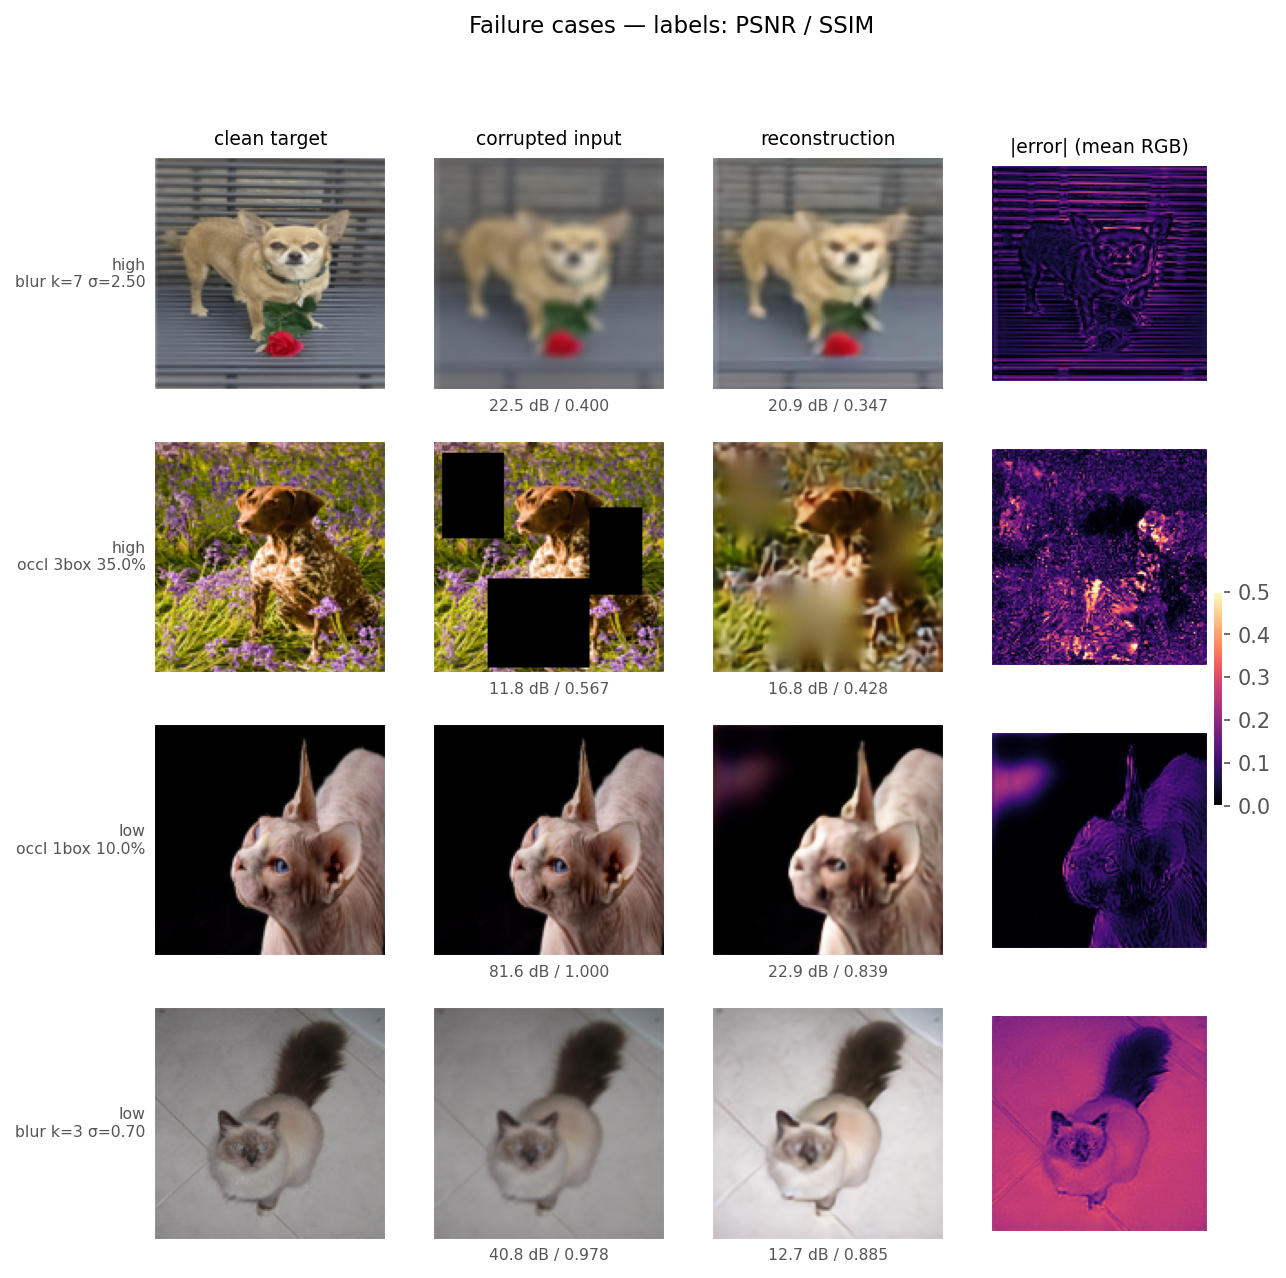
\includegraphics[width=\columnwidth]{task1/test_failure_cases.png}
    \caption{Task 1 failure cases showing difficult restoration scenarios.}
    \label{fig:t1failures}
\end{figure}

\textbf{Failure cases.} The primary failure mode is heavy occlusion covering facial features of the pet—the model hallucinates plausible but incorrect textures. For Gaussian blur at low severity, the model sometimes introduces slight artifacts where the input was already near-clean.

\subsection{Skip Connection Ablation}

\begin{table}[h]
\centering
\caption{Skip Connection Ablation Study}
\label{tab:skipablation}
\begin{tabular}{lccc}
\toprule
Variant & Code dim & PSNR & SSIM \\
\midrule
Pure AE (0 skips) & 1024 & 21.00 & 0.701 \\
1 bottlenecked skip & 2048 & 21.03 & 0.723 \\
2 bottlenecked skips & 6144 & 24.25 & 0.835 \\
2 wide skips & 295936 & 25.78 & 0.872 \\
\bottomrule
\end{tabular}
\end{table}

The selected configuration (2 bottlenecked skips, 4 channels each) achieves a compression ratio of 8:1 while retaining most of the quality of wide skips. The latent-drop test confirms the bottleneck carries essential information (5.63~dB drop), satisfying the autoencoder requirement.

\subsection{ONNX Export}

The model was exported to ONNX with a maximum absolute difference of $3.67 \times 10^{-5}$ between PyTorch and ONNX outputs. Inference latency: 67.7~ms (CPU).

% ============================================================================
\section{Task 2: Hard-Routed Specialist Restoration}

\subsection{Corruption Classifier}

A convolutional classifier predicts one of four corruption classes. The architecture uses four convolutional blocks (16-32-64-128 channels) with GroupNorm, ReLU, and max-pooling, followed by concatenated global average and max pooling and a linear classifier head.

\textbf{Design rationale.} The first block operates at full $128 \times 128$ resolution to preserve pixel-level cues (salt-and-pepper impulses, slight blur). GroupNorm is preferred over BatchNorm because it produces identical behavior in train/eval modes, which matters when the classifier is later reused as the Task~3 gating network. Concatenating global average and max pooling captures both global statistics (blur) and rare extreme activations (impulse noise, occlusion edges).

\subsubsection{Optuna Search}

\begin{table}[h]
\centering
\caption{Classifier Optuna Search Space and Best Configuration}
\label{tab:t2clfoptuna}
\begin{tabular}{lll}
\toprule
Parameter & Range & Best \\
\midrule
Learning rate & $[10^{-4}, 5 \times 10^{-3}]$ & $1.84 \times 10^{-3}$ \\
Batch size & $\{32, 64, 128\}$ & 64 \\
Channels & configs & 16-32-64-128 \\
Dropout & $[0.0, 0.5]$ & 0.155 \\
Weight decay & $[10^{-6}, 10^{-3}]$ & $2.19 \times 10^{-5}$ \\
\bottomrule
\end{tabular}
\end{table}

\subsubsection{Classifier Results}

\begin{table}[h]
\centering
\caption{Classifier Test Performance (Per-Class)}
\label{tab:t2clfresults}
\begin{tabular}{lcccc}
\toprule
Class & Precision & Recall & F1 & Support \\
\midrule
Clean & 0.998 & 0.991 & 0.994 & 3,669 \\
Salt-pepper & 1.000 & 1.000 & 1.000 & 11,007 \\
Gaussian blur & 0.999 & 1.000 & 0.999 & 11,007 \\
Occlusion & 0.998 & 0.999 & 0.999 & 11,007 \\
\midrule
Macro avg & 0.999 & 0.997 & 0.998 & 36,690 \\
\bottomrule
\end{tabular}
\end{table}

\begin{figure}[h]
    \centering
    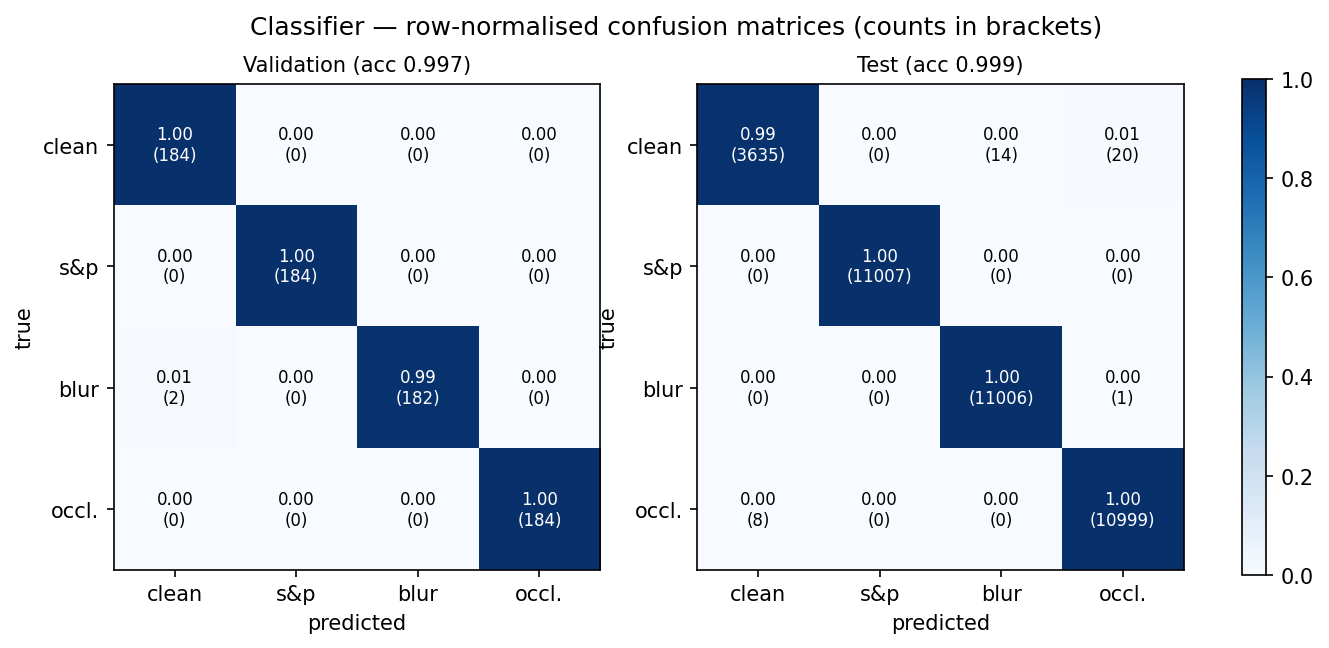
\includegraphics[width=0.75\columnwidth]{task2/classifier_confusion.png}
    \caption{Task 2 normalized confusion matrix for the corruption classifier.}
    \label{fig:t2confusion}
\end{figure}

Overall accuracy: \textbf{99.88\%}. The classifier achieves near-perfect discrimination. The only notable confusion is a small fraction (0.93\%) of clean images misclassified as other types.

\subsection{Specialist Autoencoders}

Three specialist denoising autoencoders were trained, one per corruption type, each using only its corresponding corruption data. A shared Optuna study (12+ trials) identified a common architecture: base channels 64, latent channels 8, 2 skip levels with 2 skip channels, $\alpha = 0.544$, learning rate $4.29 \times 10^{-4}$, batch size 16, dropout 0.048.

\subsection{Hard-Routed Inference Results}

\begin{table}[h]
\centering
\caption{Task 2 — Hard-Routed Test Results}
\label{tab:t2routing}
\begin{tabular}{lccc}
\toprule
Type & PSNR oracle & PSNR predicted & Routing acc \\
\midrule
Salt-pepper & 27.98 & 27.98 & 100\% \\
Gaussian blur & 24.92 & 24.92 & 99.99\% \\
Occlusion & 21.68 & 21.68 & 99.93\% \\
\midrule
All corrupted & 24.86 & 24.86 & 99.97\% \\
\bottomrule
\end{tabular}
\end{table}

The gap between oracle and predicted routing is negligible ($\Delta$PSNR = 0.002~dB), confirming that classifier errors have minimal impact on restoration quality. Only 0.12\% of images were misrouted.

\begin{figure}[h]
    \centering
    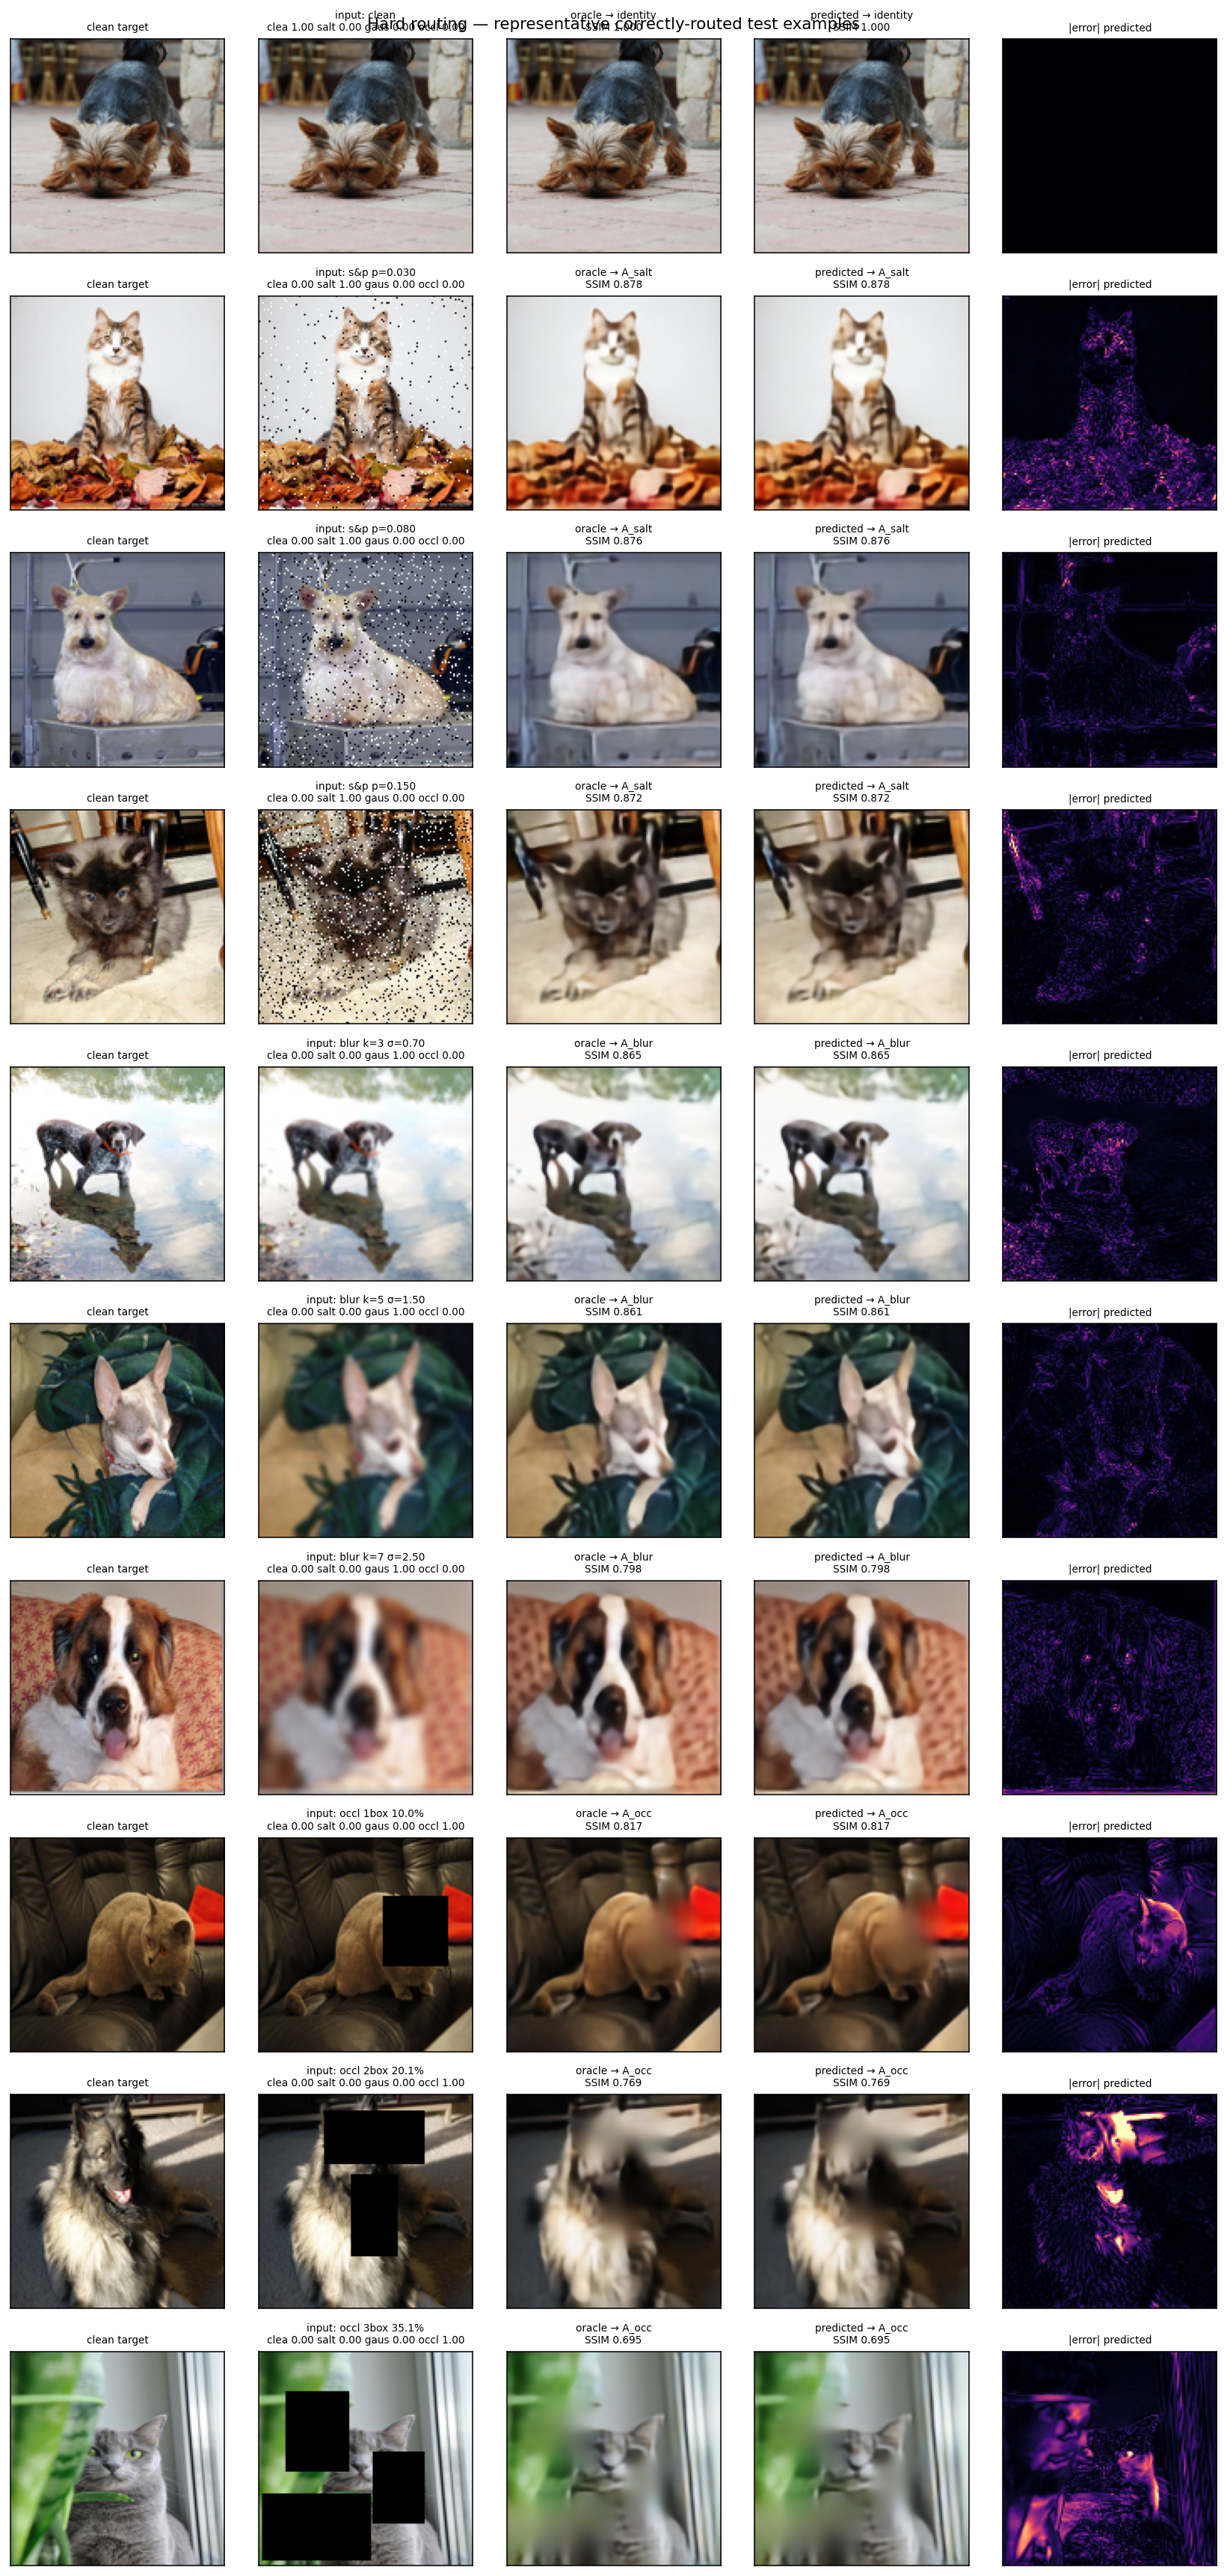
\includegraphics[width=\columnwidth]{task2/routing_representative.png}
    \caption{Task 2 hard-routed restoration examples showing classifier prediction and specialist output.}
    \label{fig:t2examples}
\end{figure}

\begin{figure}[h]
    \centering
    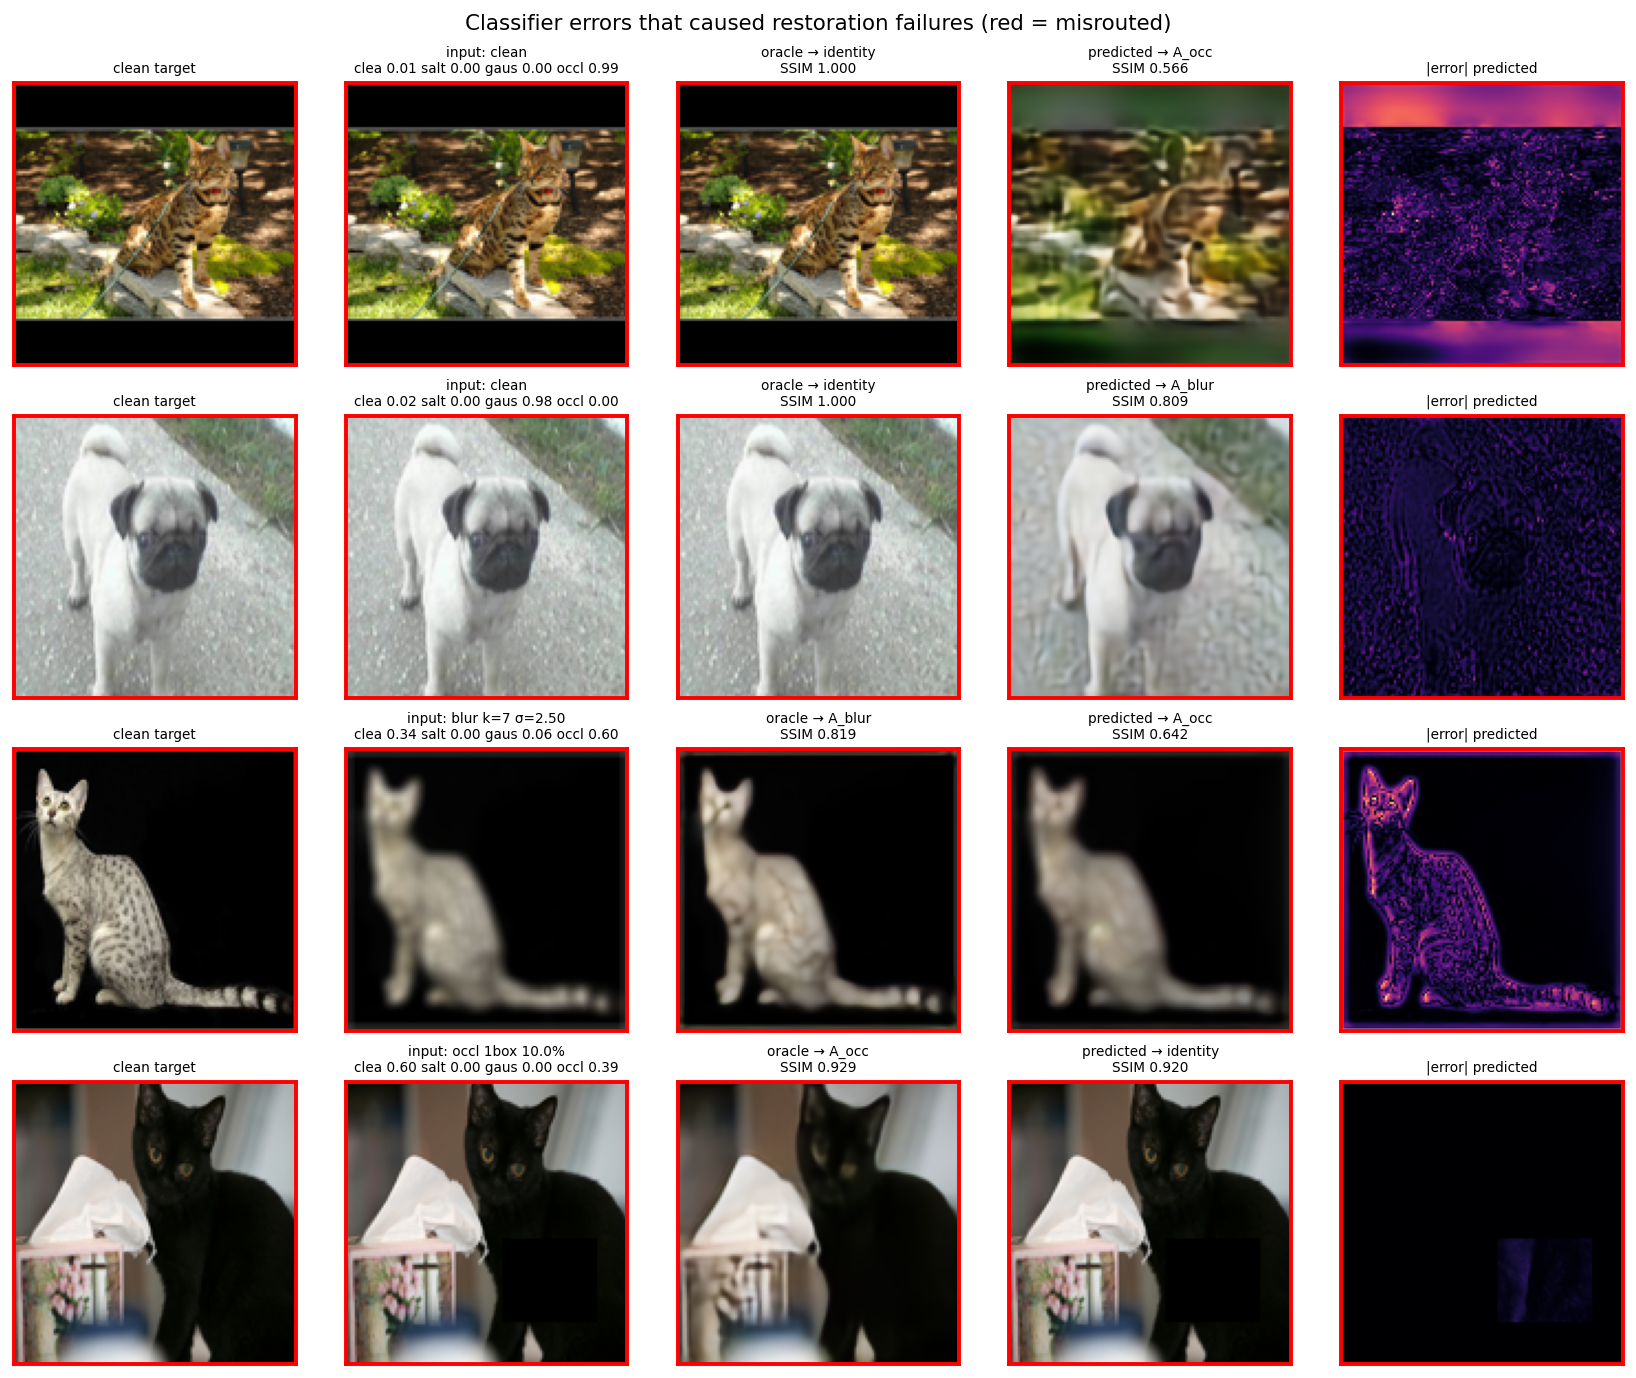
\includegraphics[width=\columnwidth]{task2/misrouting_failures.png}
    \caption{Task 2 misrouting failure cases where classifier errors led to incorrect specialist selection.}
    \label{fig:t2failures}
\end{figure}

Clean images use an identity bypass (99.07\% correctly identified as clean). The remaining 0.93\% are unnecessarily processed by a specialist, producing slight quality reduction (24.48~dB vs.\ lossless identity).

\textbf{Comparison with Task~1.} The specialist approach achieves 24.86~dB vs.\ the universal model's 24.72~dB (+0.14~dB). The advantage is modest because the universal model already learned effective corruption-specific features. However, the salt-and-pepper specialist significantly outperforms the universal model (27.98 vs.\ 26.73~dB).

% ============================================================================
\section{Task 3: Soft Mixture-of-Experts Restoration}

\subsection{Architecture}

The soft MoE system replaces hard routing with differentiable weighted blending:
\begin{equation}
    w = \text{softmax}\left(\frac{G(\tilde{x})}{\tau}\right), \quad
    \hat{x} = w_0 \tilde{x} + \sum_{k=1}^{3} w_k A_k(\tilde{x})
\end{equation}

The gating network $G$ is initialized from the Task~2 classifier, and the three experts from the Task~2 specialists.

\subsection{Joint Training Procedure}

\begin{enumerate}
    \item \textbf{Warm-up} (experts frozen): only the gate is trained to adapt to soft routing.
    \item \textbf{Joint fine-tuning}: all parameters are unfrozen with a reduced learning rate.
\end{enumerate}

The joint loss combines four terms:
\begin{equation}
    \mathcal{L}_{\text{MoE}} = \lambda_1 \mathcal{L}_{\text{L1}} + \lambda_s (1 - \text{SSIM}) + \lambda_c \mathcal{L}_{\text{CE}} + \lambda_b \mathcal{L}_{\text{balance}}
\end{equation}

The balance loss prevents routing collapse:
\begin{equation}
    \mathcal{L}_{\text{balance}} = \sum_{k=0}^{3}\left(\bar{w}_k - \frac{1}{4}\right)^2
\end{equation}

\subsection{Optuna Search}

\begin{table}[h]
\centering
\caption{Task 3 Optuna Search Space and Best Configuration}
\label{tab:t3optuna}
\begin{tabular}{lll}
\toprule
Parameter & Range & Best \\
\midrule
Joint LR & $[10^{-5}, 3 \times 10^{-4}]$ (log) & $1.59 \times 10^{-5}$ \\
$\tau$ (temperature) & $[0.5, 3.0]$ (log) & 1.063 \\
$\alpha$ (L1 weight) & $[0.5, 0.95]$ & 0.518 \\
$\lambda_c$ (CE weight) & $[0.01, 1.0]$ (log) & 0.014 \\
$\lambda_b$ (balance weight) & $[0.001, 0.3]$ (log) & 0.009 \\
\bottomrule
\end{tabular}
\end{table}

15 trials completed. The selected temperature ($\tau \approx 1.06$) is near unity, indicating the gate logits are already well-calibrated from the Task~2 classifier initialization. The low $\lambda_c$ and $\lambda_b$ values suggest reconstruction quality dominates the objective.

\subsection{Routing Behavior}

\begin{table}[h]
\centering
\caption{Average Routing Weights by Corruption Type}
\label{tab:t3routing}
\begin{tabular}{lcccc}
\toprule
Type & Identity & A\_salt & A\_blur & A\_occ \\
\midrule
Clean & 0.989 & 0.000 & 0.009 & 0.002 \\
Salt-pepper & 0.015 & 0.985 & 0.000 & 0.000 \\
Gaussian blur & 0.362 & 0.000 & 0.637 & 0.001 \\
Occlusion & 0.246 & 0.000 & 0.001 & 0.753 \\
\bottomrule
\end{tabular}
\end{table}

\textbf{Analysis.} Clean images are routed almost entirely to the identity branch (98.9\%). Salt-and-pepper routing is sharp (98.5\% to the salt expert). Gaussian blur distributes 36.2\% weight to identity and 63.7\% to the blur expert—this is sensible because mildly blurred images are close to clean. Occlusion follows a similar pattern with 24.6\% identity weight, reflecting that unoccluded regions need no processing.

\begin{figure}[h]
    \centering
    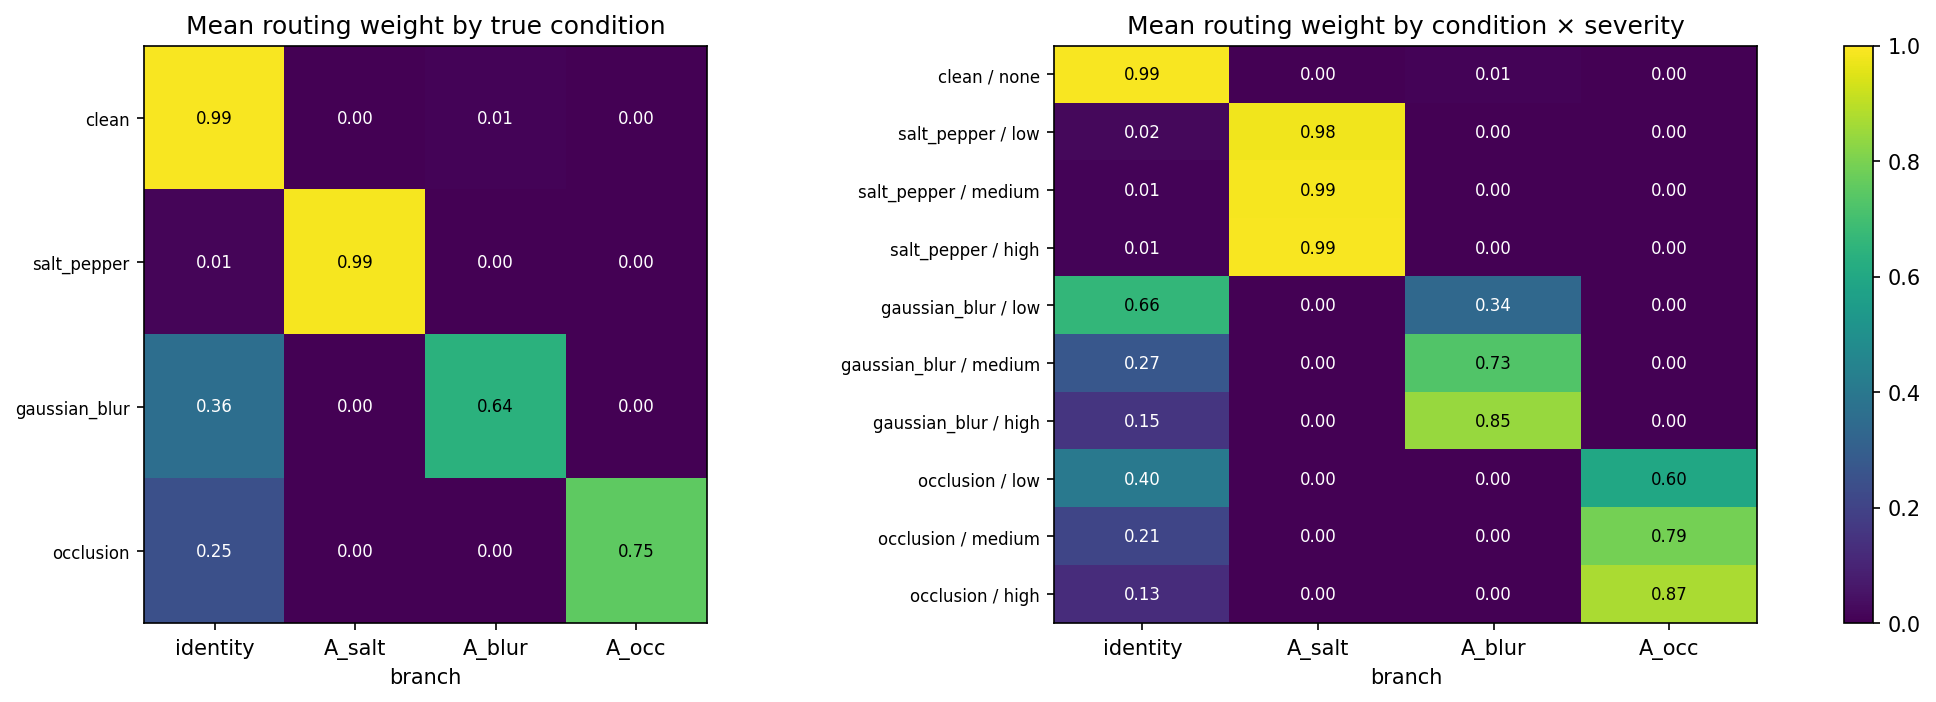
\includegraphics[width=\columnwidth]{task3/routing_heatmap.png}
    \caption{Task 3 routing weight heatmap showing average expert weights per corruption type and severity.}
    \label{fig:t3heatmap}
\end{figure}

\begin{figure}[h]
    \centering
    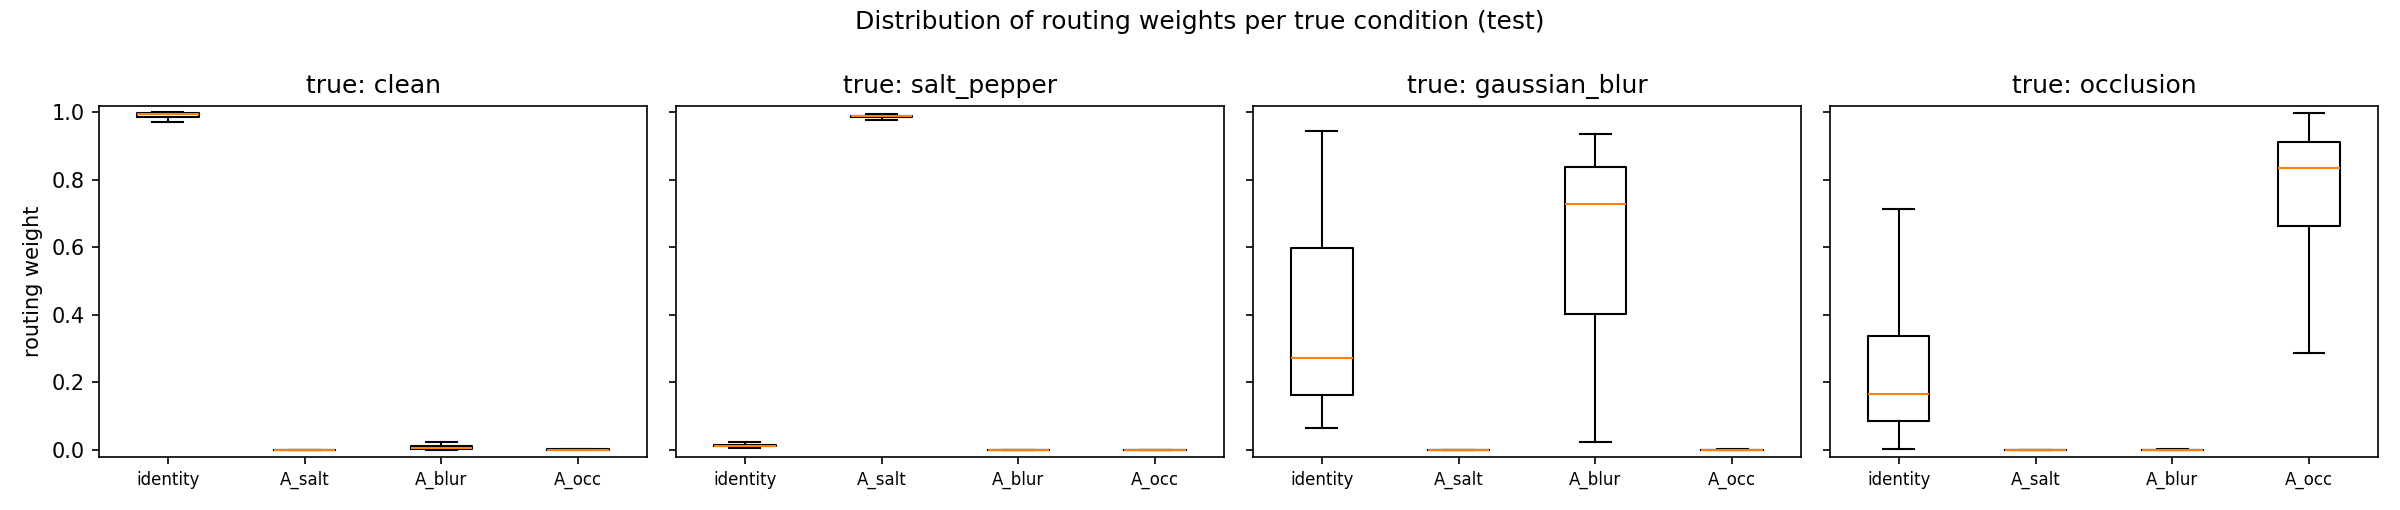
\includegraphics[width=\columnwidth]{task3/routing_weight_distributions.png}
    \caption{Task 3 routing weight distributions across the test set.}
    \label{fig:t3distributions}
\end{figure}

Expert usage across the dataset: identity 28.6\%, salt 29.6\%, blur 19.2\%, occlusion 22.6\%. No expert is inactive, though the blur expert receives less traffic because the gate shares load with the identity branch for mild blur.

\subsection{Results}

\begin{table}[h]
\centering
\caption{Task 3 — Soft MoE vs.\ Hard Routing vs.\ Universal}
\label{tab:t3comparison}
\begin{tabular}{lccc}
\toprule
Method & PSNR & SSIM & Gate/Clf acc \\
\midrule
Universal (T1) & 24.72 & 0.838 & — \\
Hard-routed (T2) & 24.86 & 0.812 & 99.97\% \\
\textbf{Soft MoE (T3)} & \textbf{25.59} & \textbf{0.835} & 84.79\% \\
\bottomrule
\end{tabular}
\end{table}

The soft MoE achieves the highest PSNR (+0.73~dB over hard routing, +0.87~dB over universal). Although the gate ``accuracy'' drops to 84.8\%, this is expected: the gate learned to distribute weights rather than make hard decisions, and the distributed routing produces better reconstruction.

\begin{figure}[h]
    \centering
    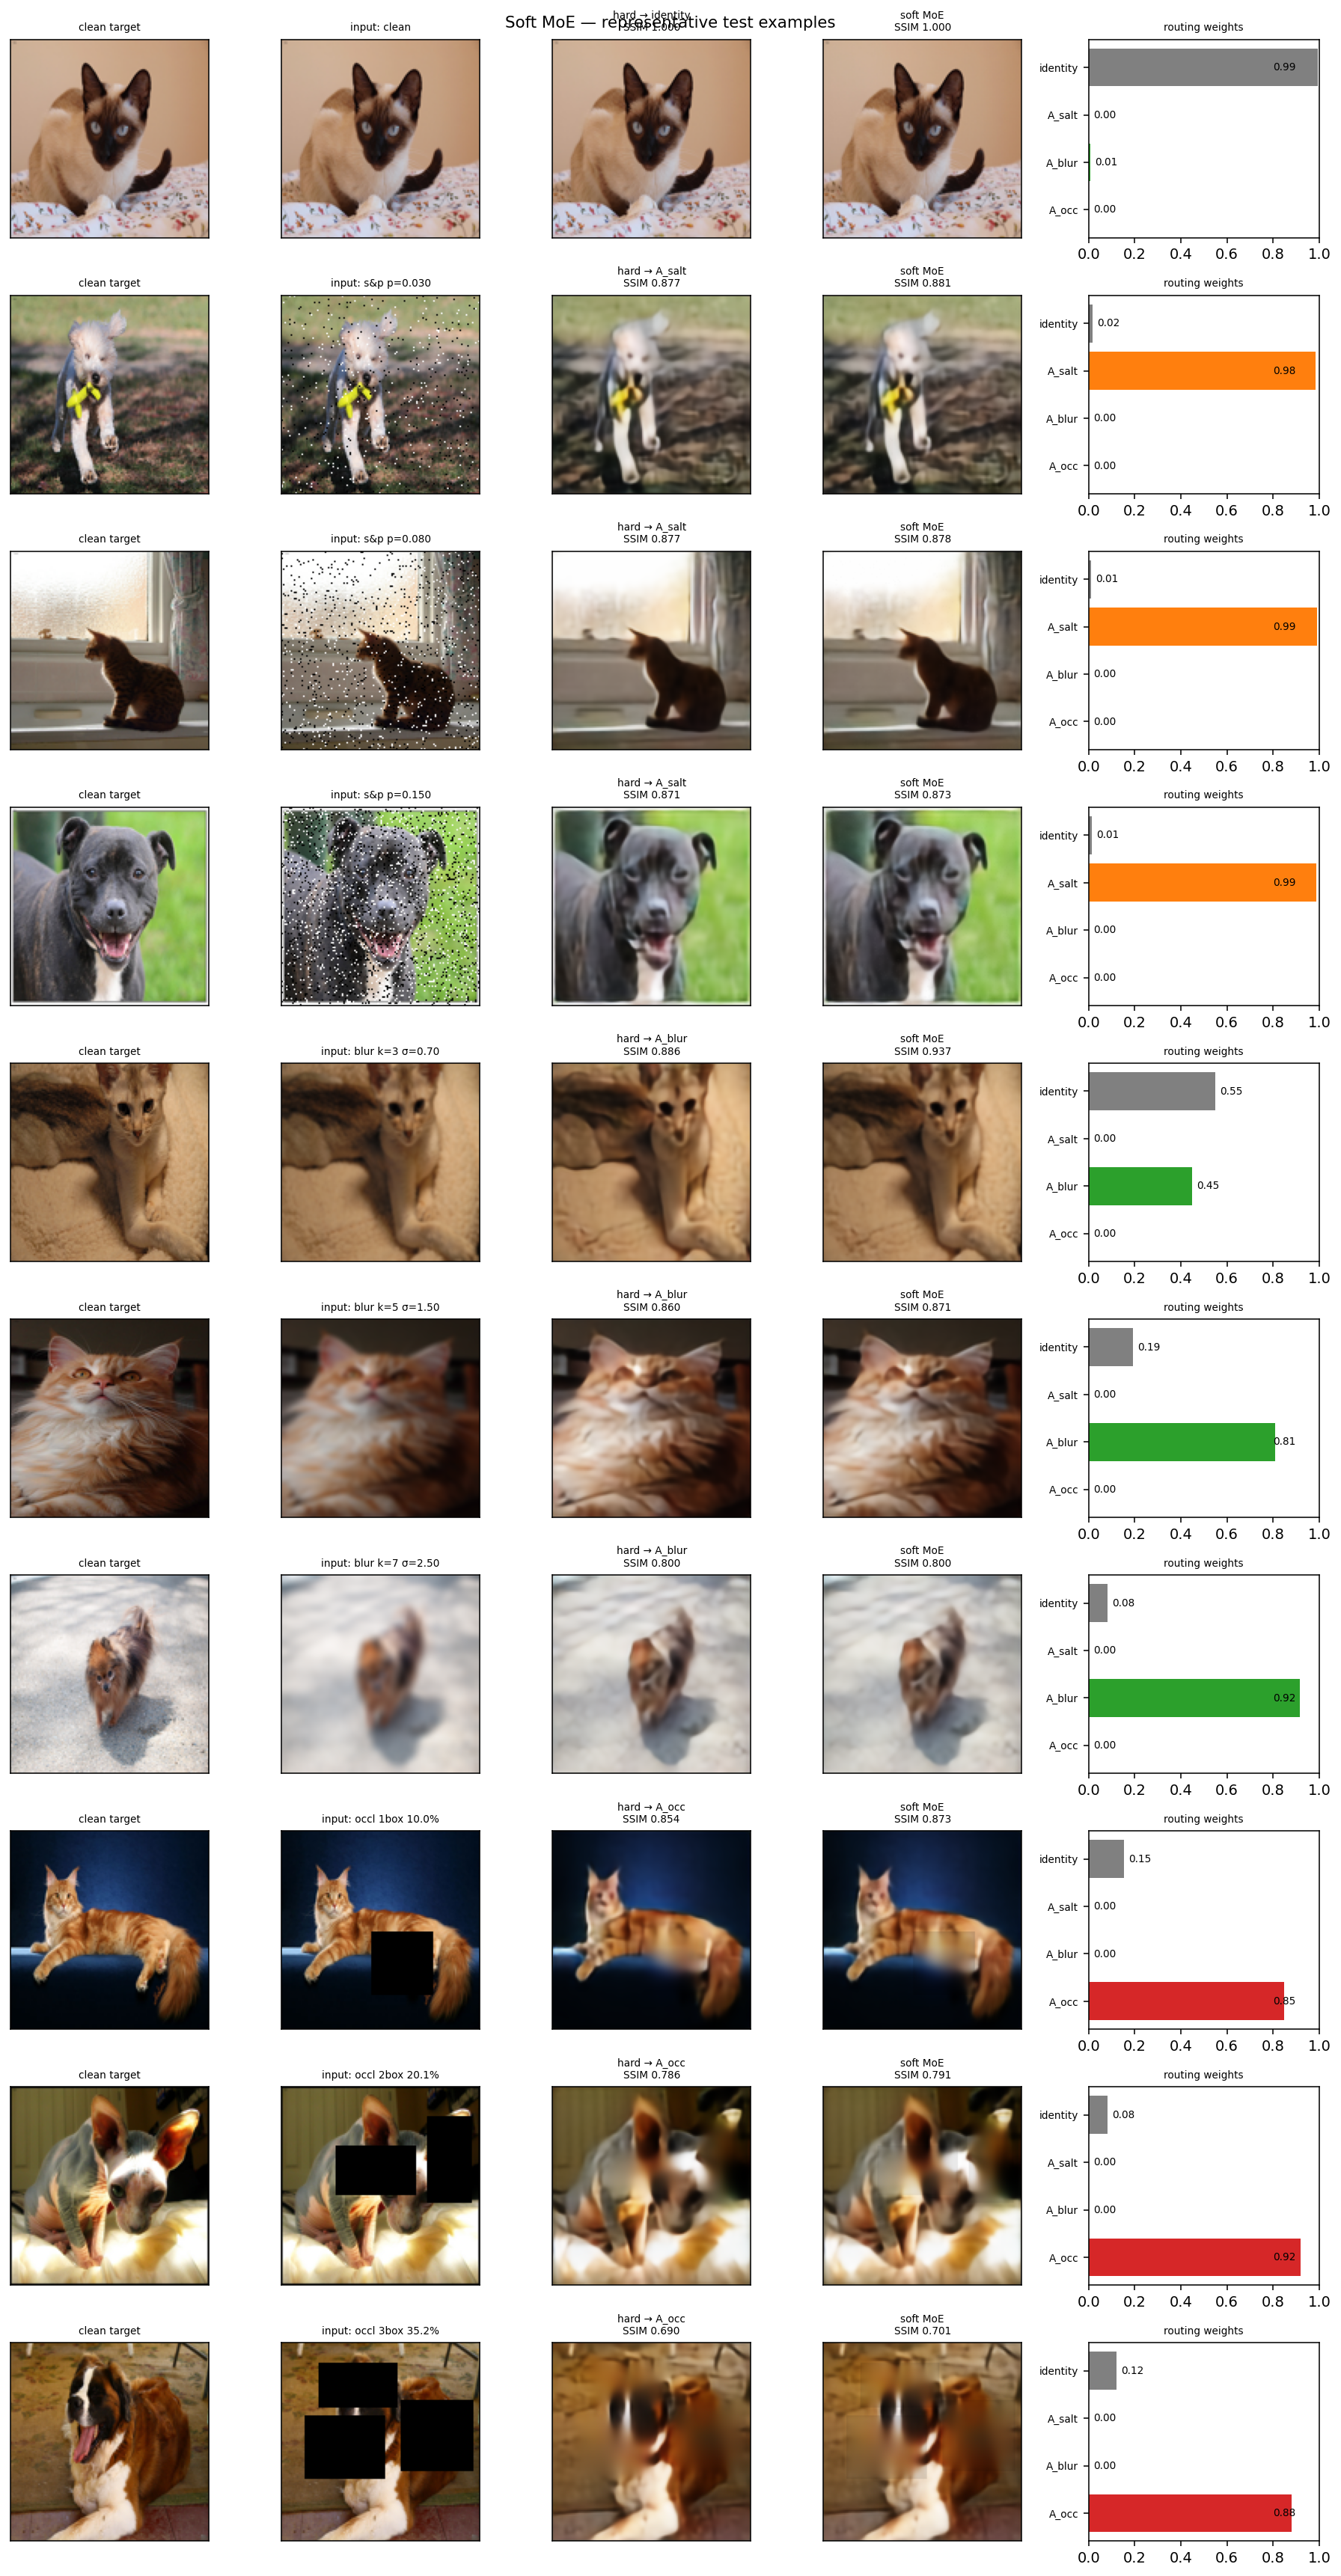
\includegraphics[width=\columnwidth]{task3/examples_representative.png}
    \caption{Task 3 representative soft MoE restoration results.}
    \label{fig:t3examples}
\end{figure}

\begin{figure}[h]
    \centering
    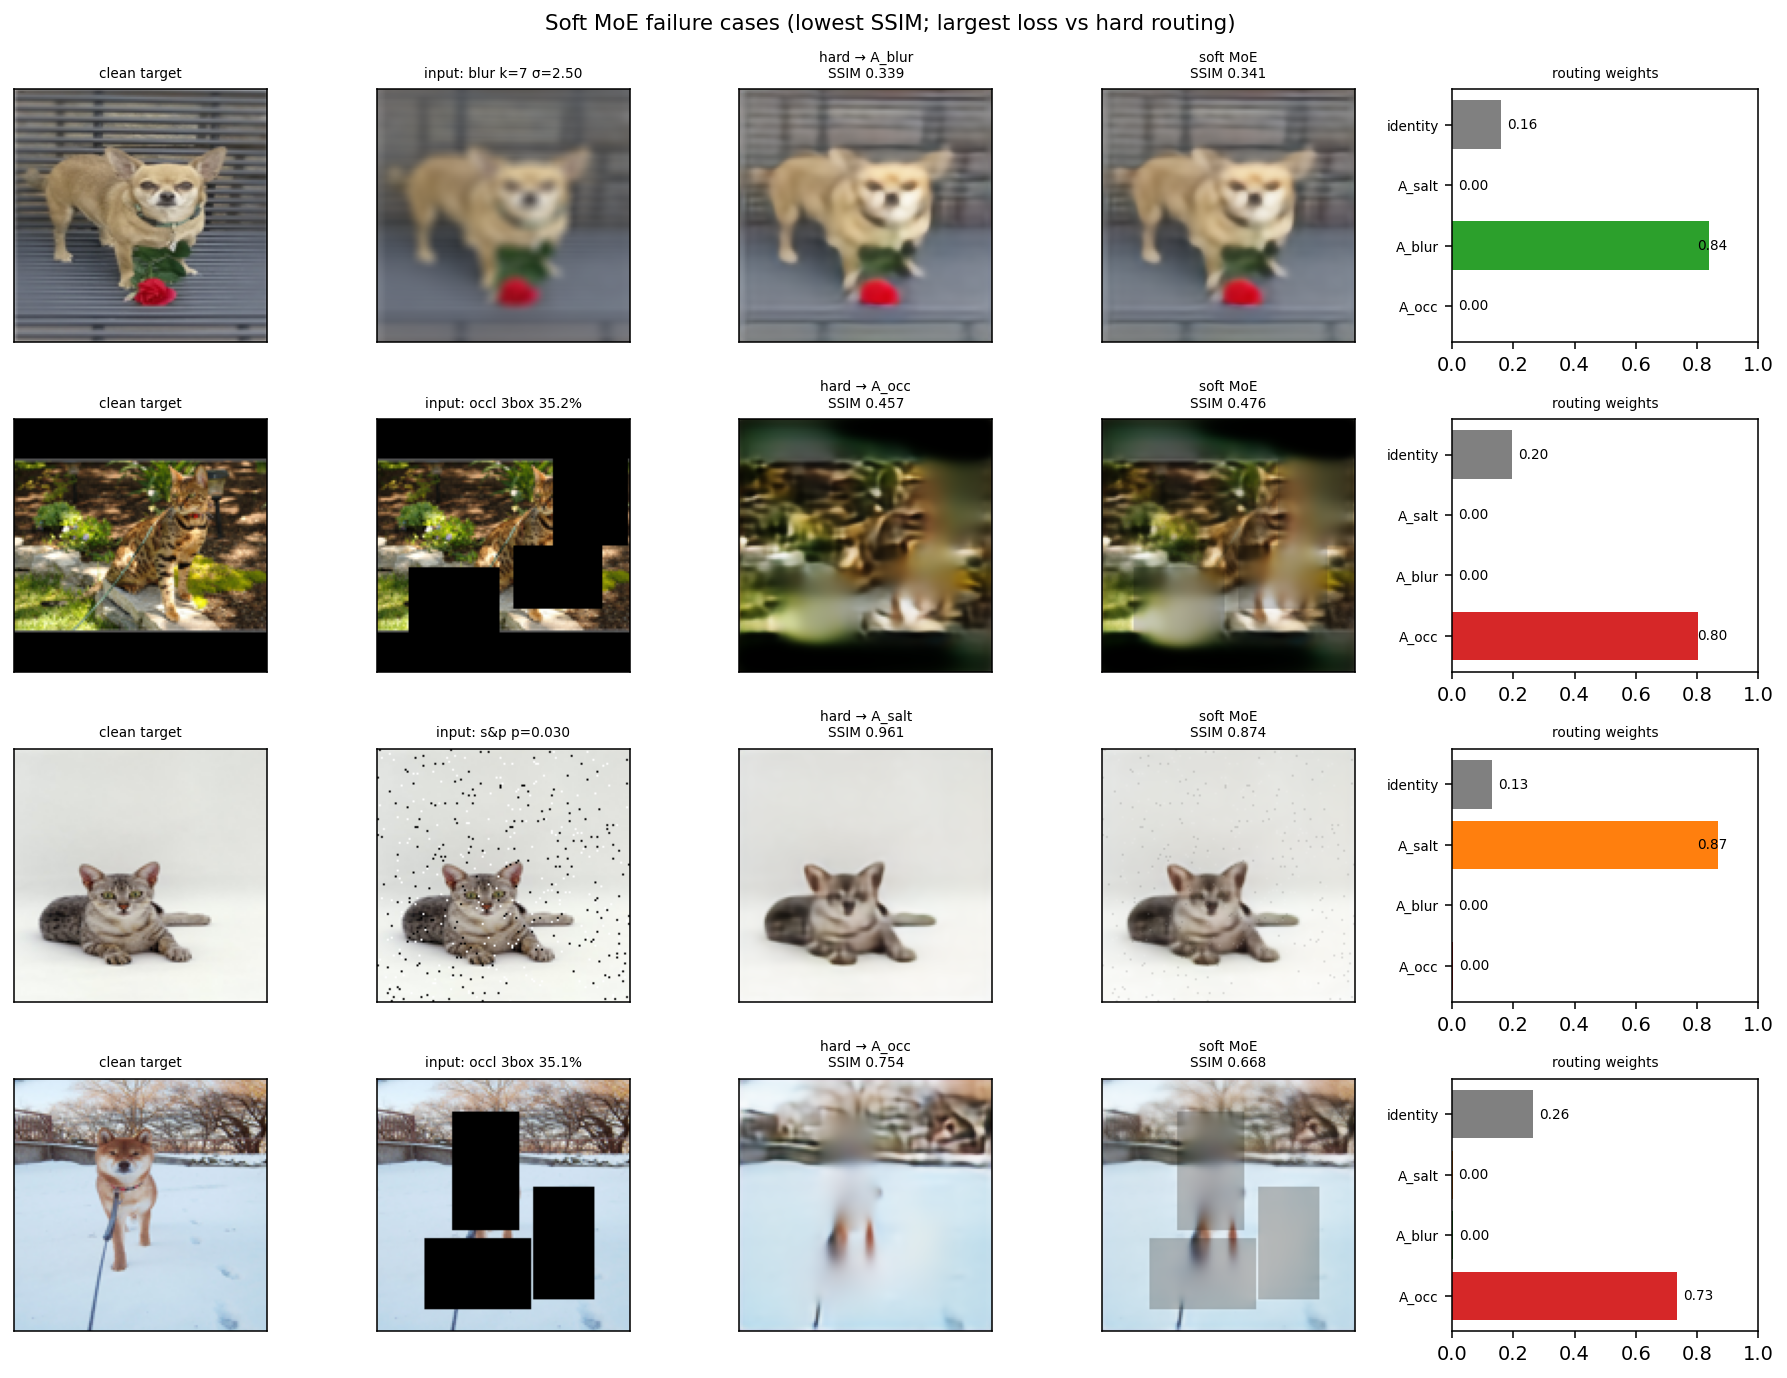
\includegraphics[width=\columnwidth]{task3/examples_failures.png}
    \caption{Task 3 failure cases for the soft MoE system.}
    \label{fig:t3failures}
\end{figure}

\textbf{Compound corruptions.} On images with two simultaneous corruptions (not seen during training), the soft MoE outperforms hard routing for salt-pepper + Gaussian blur ($\Delta$SSIM = 0.005) and slightly underperforms for other combinations, demonstrating partial generalization to compound degradations.

% ============================================================================
\section{Task 4: Style-Conditioned Face-to-Sketch Generation}

\subsection{Architecture}

\textbf{Generator.} A U-Net encoder-decoder with skip connections. The style condition is a learned 32-dimensional embedding incorporated via:
\begin{itemize}
    \item Concatenation at the $1 \times 1$ bottleneck.
    \item Conditional Instance Normalization (CIN) in every decoder block, where per-style $\gamma$ and $\beta$ affine parameters modulate features (Dumoulin et al.\ 2017).
\end{itemize}

\textbf{Discriminator.} A PatchGAN discriminator that receives the concatenation of photograph, sketch, and a spatially broadcast style embedding. It produces per-patch real/fake predictions.

\subsection{Loss Functions}

\begin{align}
    \mathcal{L}_G &= \mathcal{L}_{\text{adv}} + \lambda_{\text{L1}} \cdot \mathcal{L}_{\text{L1}}(y, G(x, s)) \\
    \mathcal{L}_D &= \frac{1}{2}\left[\text{BCE}(D(x, y, s), 1) + \text{BCE}(D(x, G(x,s), s), 0)\right]
\end{align}

\subsection{Optuna Search}

\begin{table}[h]
\centering
\caption{Task 4 Optuna Search Space and Best Configuration}
\label{tab:t4optuna}
\begin{tabular}{lll}
\toprule
Parameter & Range & Best \\
\midrule
Generator LR & $[5 \times 10^{-5}, 5 \times 10^{-4}]$ & $2.79 \times 10^{-4}$ \\
Discriminator LR & $[5 \times 10^{-5}, 5 \times 10^{-4}]$ & $1.74 \times 10^{-4}$ \\
Batch size & $\{4, 8, 16\}$ & 4 \\
Base channels & $\{32, 48, 64\}$ & 64 \\
Dropout & $[0.0, 0.5]$ & 0.015 \\
Embedding dim & $\{8, 16, 32\}$ & 32 \\
$\lambda_{\text{L1}}$ & $[10, 200]$ (log) & 169.0 \\
\bottomrule
\end{tabular}
\end{table}

12 trials completed, 8 pruned. The high $\lambda_{\text{L1}}$ (169) emphasizes reconstruction fidelity, consistent with pix2pix practice. The small batch size (4) provides sufficient gradient noise for GAN training stability.

\subsection{Results}

\begin{table}[h]
\centering
\caption{Task 4 — Test Metrics by Style}
\label{tab:t4results}
\begin{tabular}{lccccc}
\toprule
Style & PSNR & SSIM & LPIPS$\downarrow$ & FID$\downarrow$ & $n$ \\
\midrule
Style 1 & 16.62 & 0.488 & 0.214 & 42.22 & 619 \\
Style 2 & 11.71 & 0.366 & 0.194 & 37.67 & 381 \\
Style 3 & 18.04 & 0.606 & 0.139 & 66.90 & 46 \\
\midrule
All & 14.90 & 0.449 & 0.203 & 33.29 & 1,046 \\
\bottomrule
\end{tabular}
\end{table}

\begin{figure}[h]
    \centering
    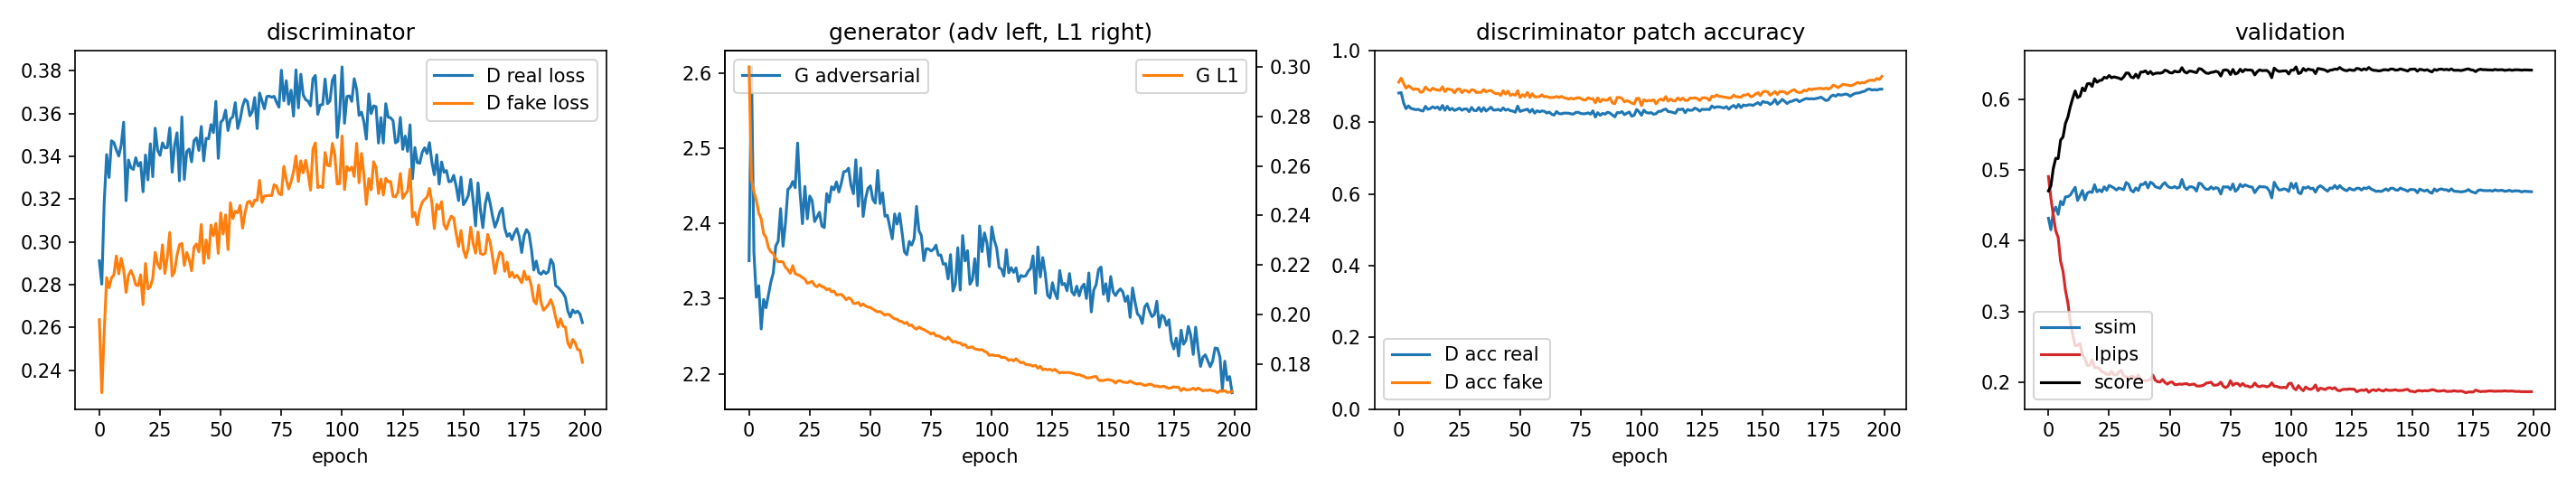
\includegraphics[width=\columnwidth]{task4/training_curves.png}
    \caption{Task 4 GAN training curves: discriminator and generator losses.}
    \label{fig:t4curves}
\end{figure}

\begin{figure}[h]
    \centering
    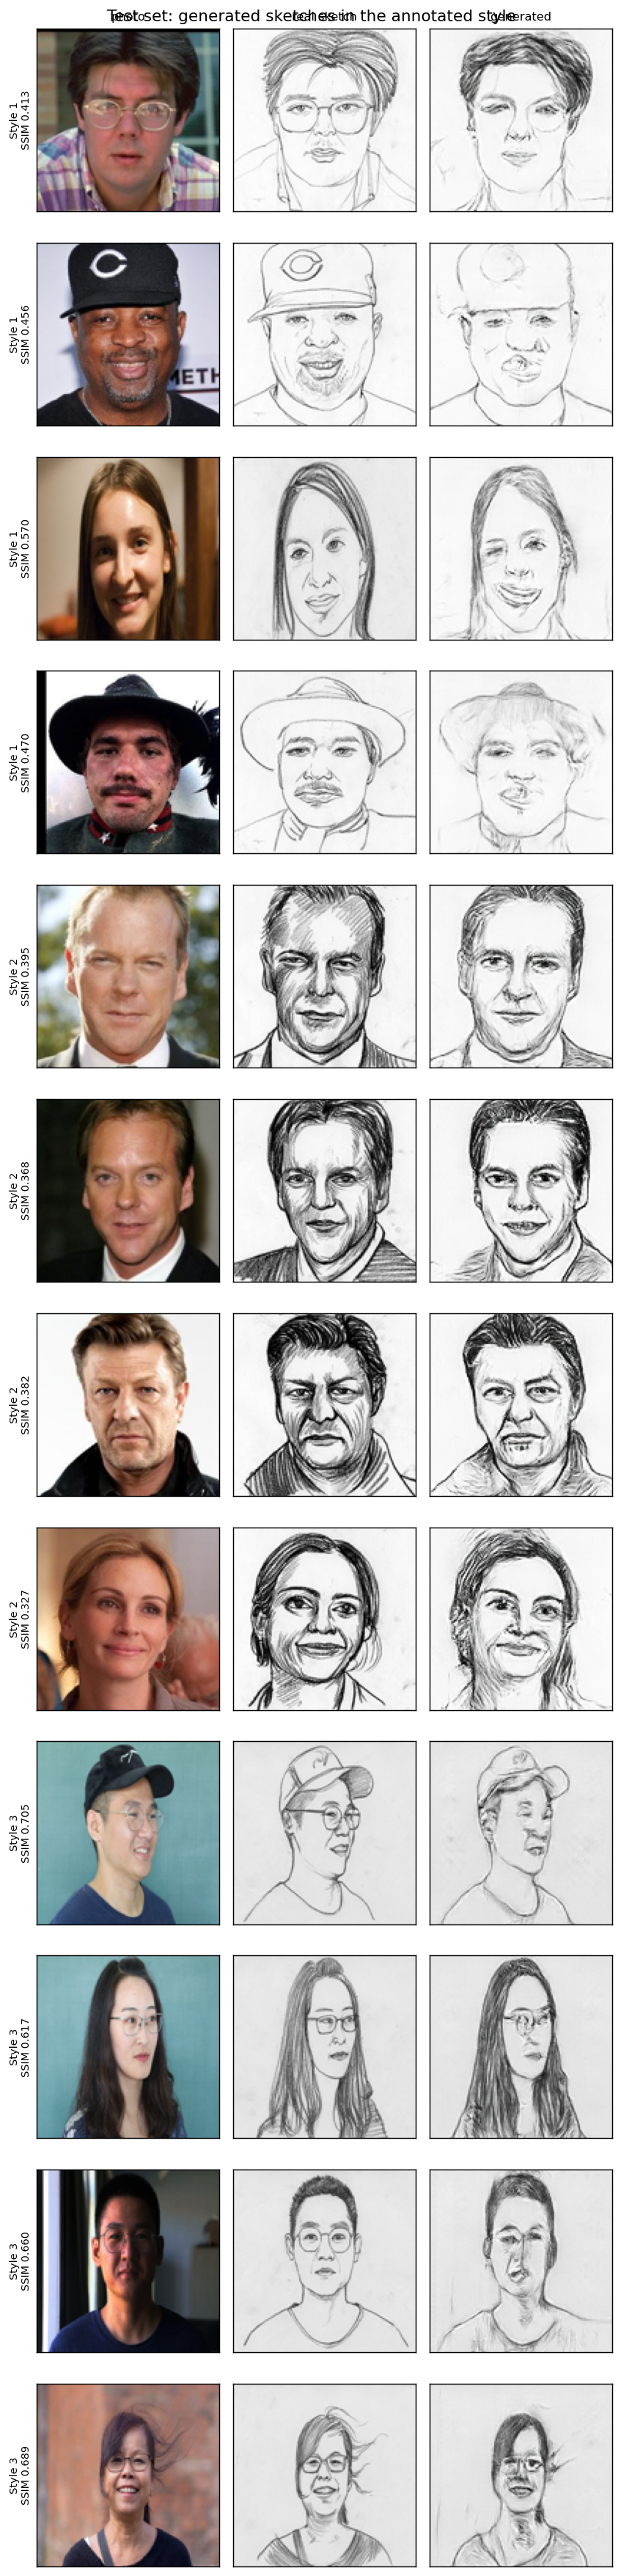
\includegraphics[width=\columnwidth]{task4/test_examples.png}
    \caption{Task 4 test results: input photograph, generated sketch, and ground-truth sketch.}
    \label{fig:t4examples}
\end{figure}

\begin{figure}[h]
    \centering
    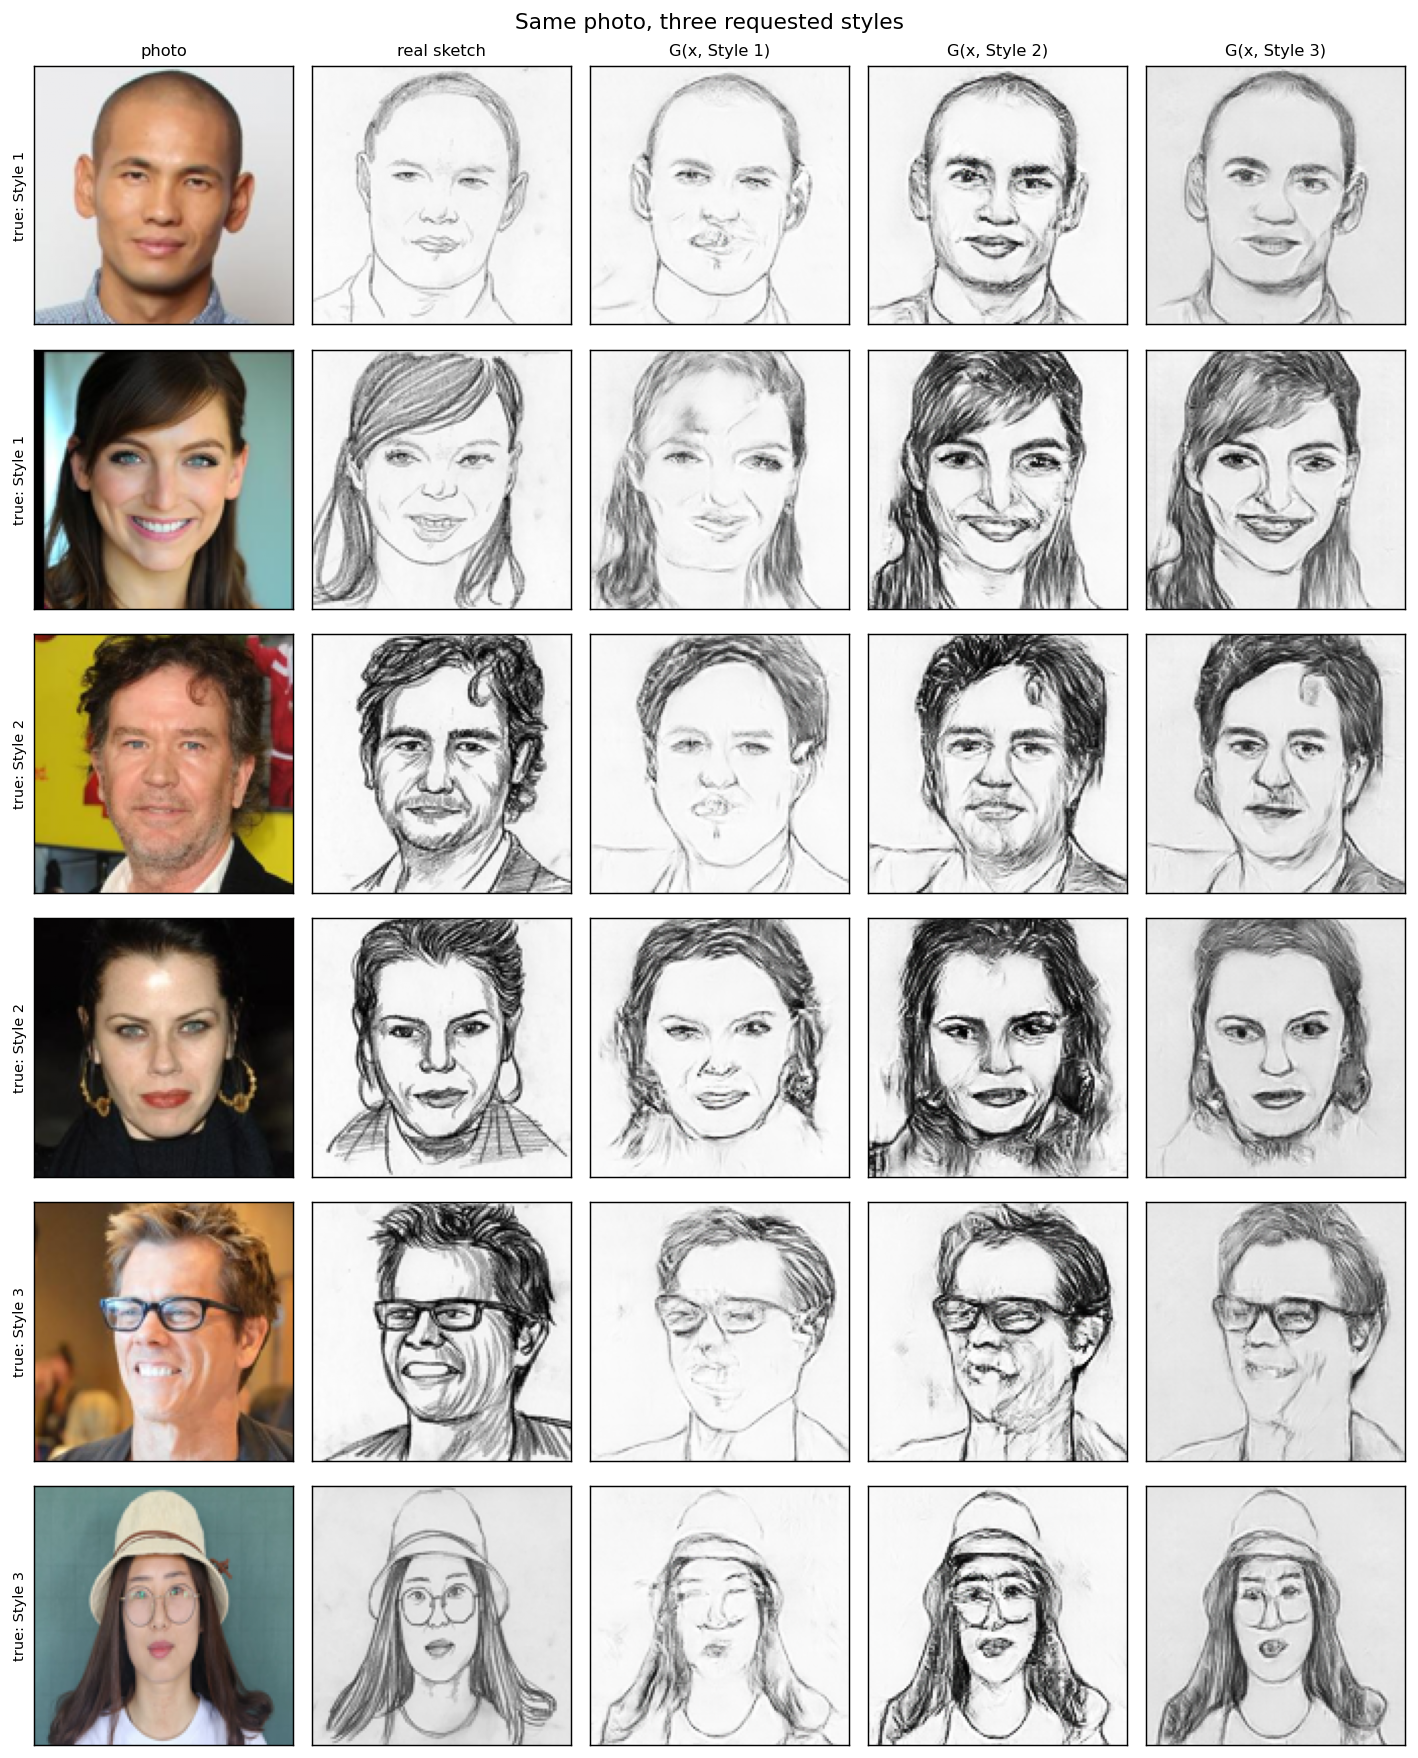
\includegraphics[width=\columnwidth]{task4/style_swap.png}
    \caption{Task 4 style-swap experiment: same photograph rendered in all three sketch styles.}
    \label{fig:t4swap}
\end{figure}

\textbf{Analysis.} Style~3 achieves the highest pixel-level metrics (PSNR 18.04, SSIM 0.606) but the worst FID (66.90), likely due to limited training data (only 46 test samples). Style~2 has lower pixel metrics but better FID, suggesting more diverse but less pixel-aligned sketches.

\textbf{Style consistency.} A style classifier trained on the generated sketches achieves 99.1\% accuracy on style assignment, confirming the generator respects the style condition. Style-swap experiments (generating the same face with all three styles) show visually distinct outputs with 94.5\% cross-style consistency.

\begin{figure}[h]
    \centering
    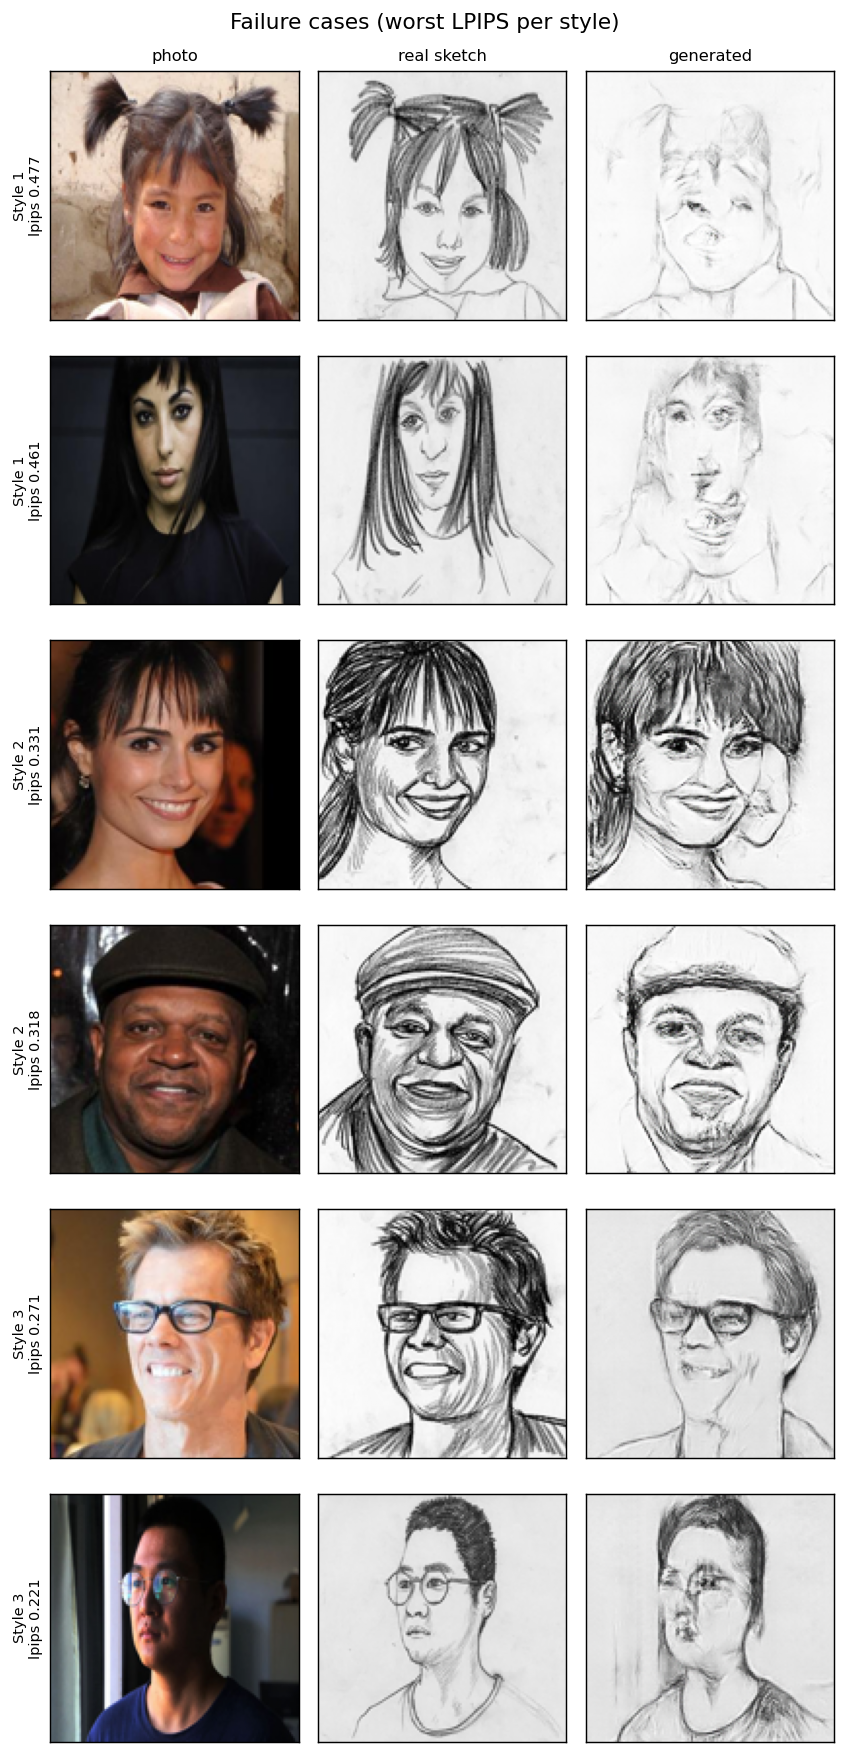
\includegraphics[width=\columnwidth]{task4/test_failures.png}
    \caption{Task 4 failure cases for face-to-sketch generation.}
    \label{fig:t4failures}
\end{figure}

\textbf{Failure cases.} The generator struggles with extreme poses (profile views), heavy occlusion of facial features (sunglasses, hands covering face), and unusual lighting conditions. Style~2 sketches occasionally lose fine detail in hair regions.

\subsection{ONNX Export}

Only the generator is exported for inference. Model size: 168.9~MB. ONNX parity verified.

% ============================================================================
\section{Application Architecture}

\subsection{UI Design}

The application interface was designed in Google Stitch before implementation. Evidence of the original Stitch designs is provided in the \texttt{Designs/} directory, with screenshots included below. The designs cover all four workspaces: Universal Restoration, Hard-Routed Restoration, Soft Mixture-of-Experts, and Face-to-Sketch Generator.

\begin{figure}[h]
    \centering
    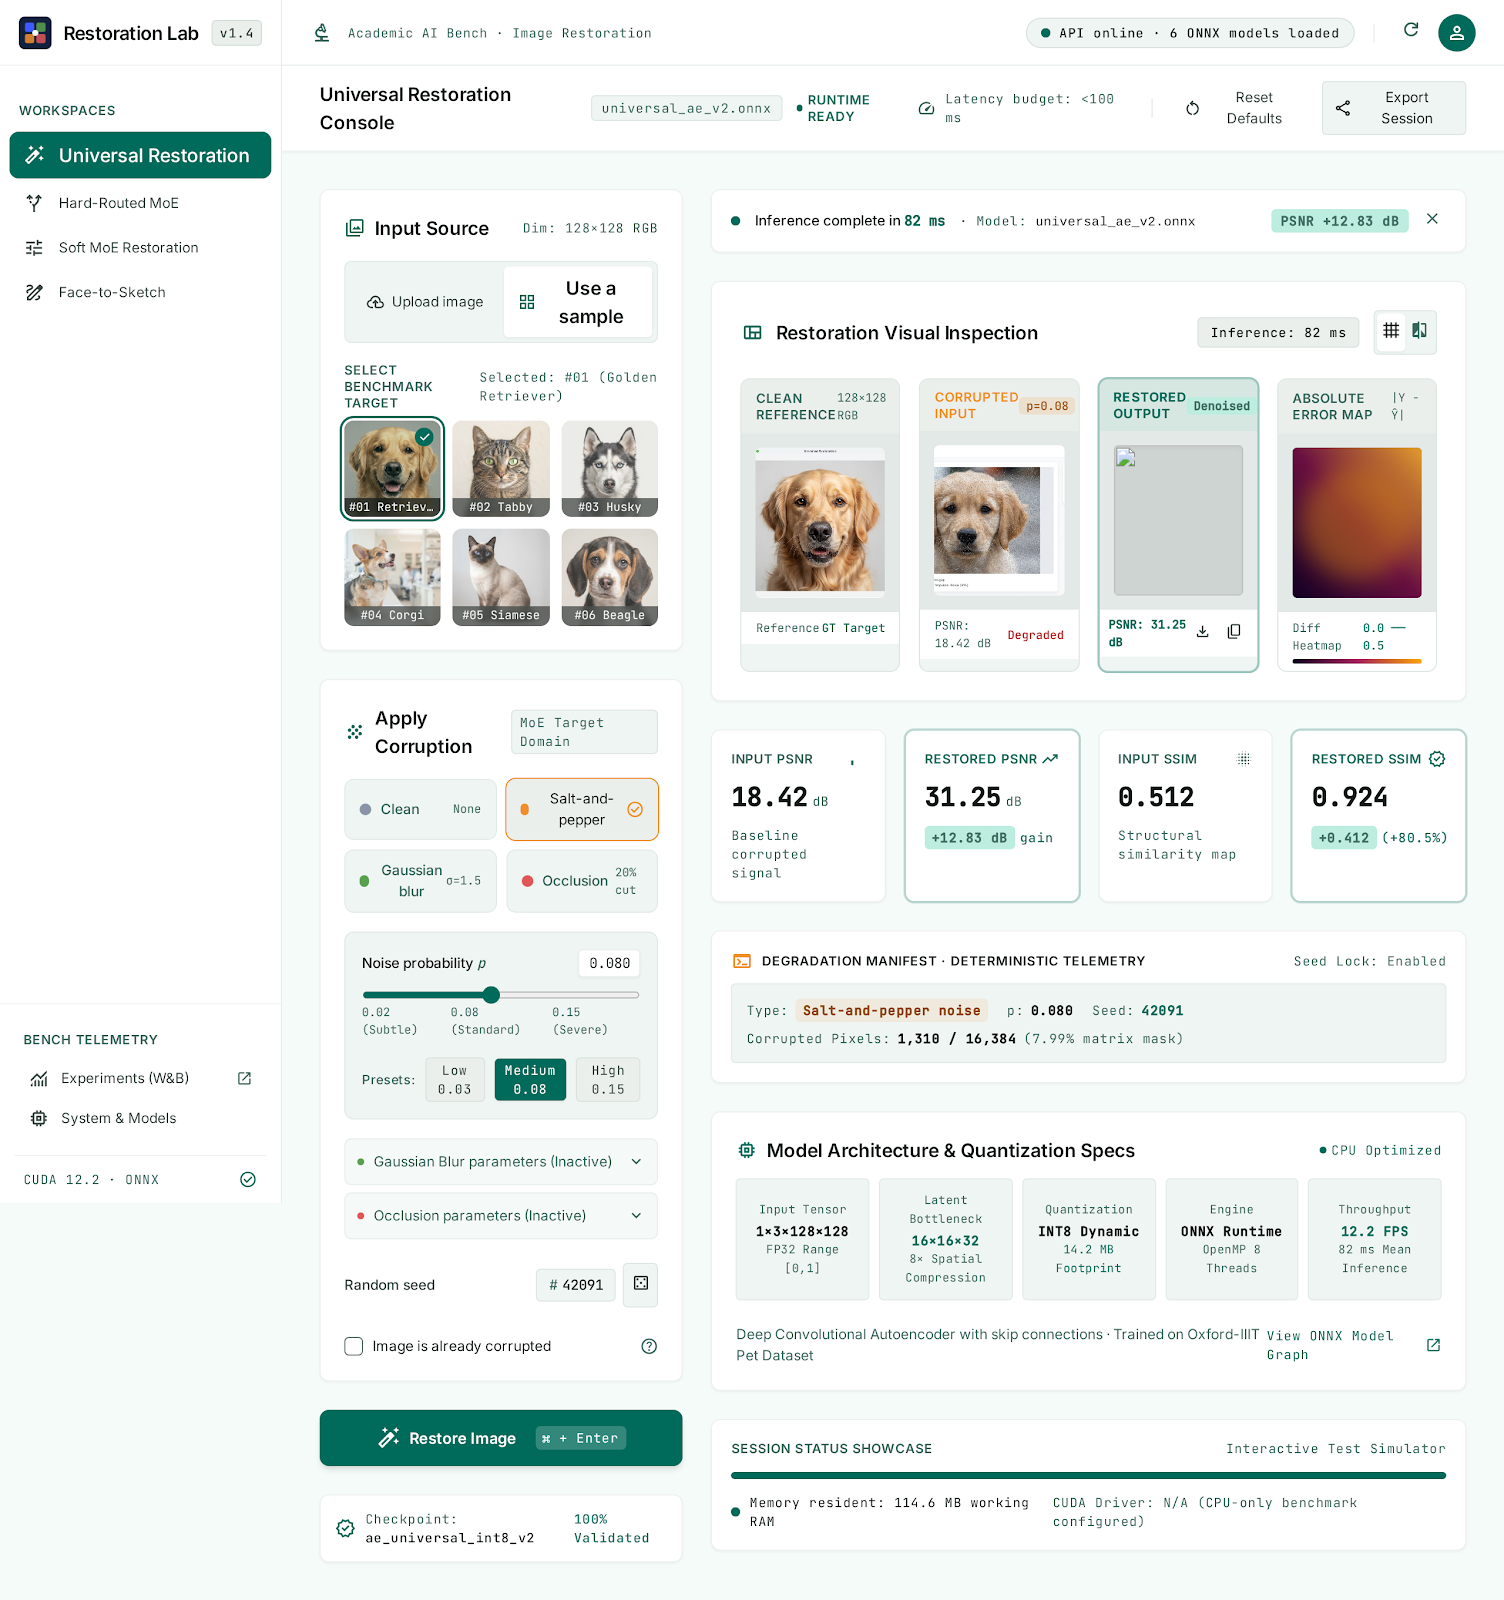
\includegraphics[width=\columnwidth]{universal-restoration/screen.png}
    \caption{Google Stitch design for Universal Restoration workspace.}
    \label{fig:stitch_universal}
\end{figure}

\begin{figure}[h]
    \centering
    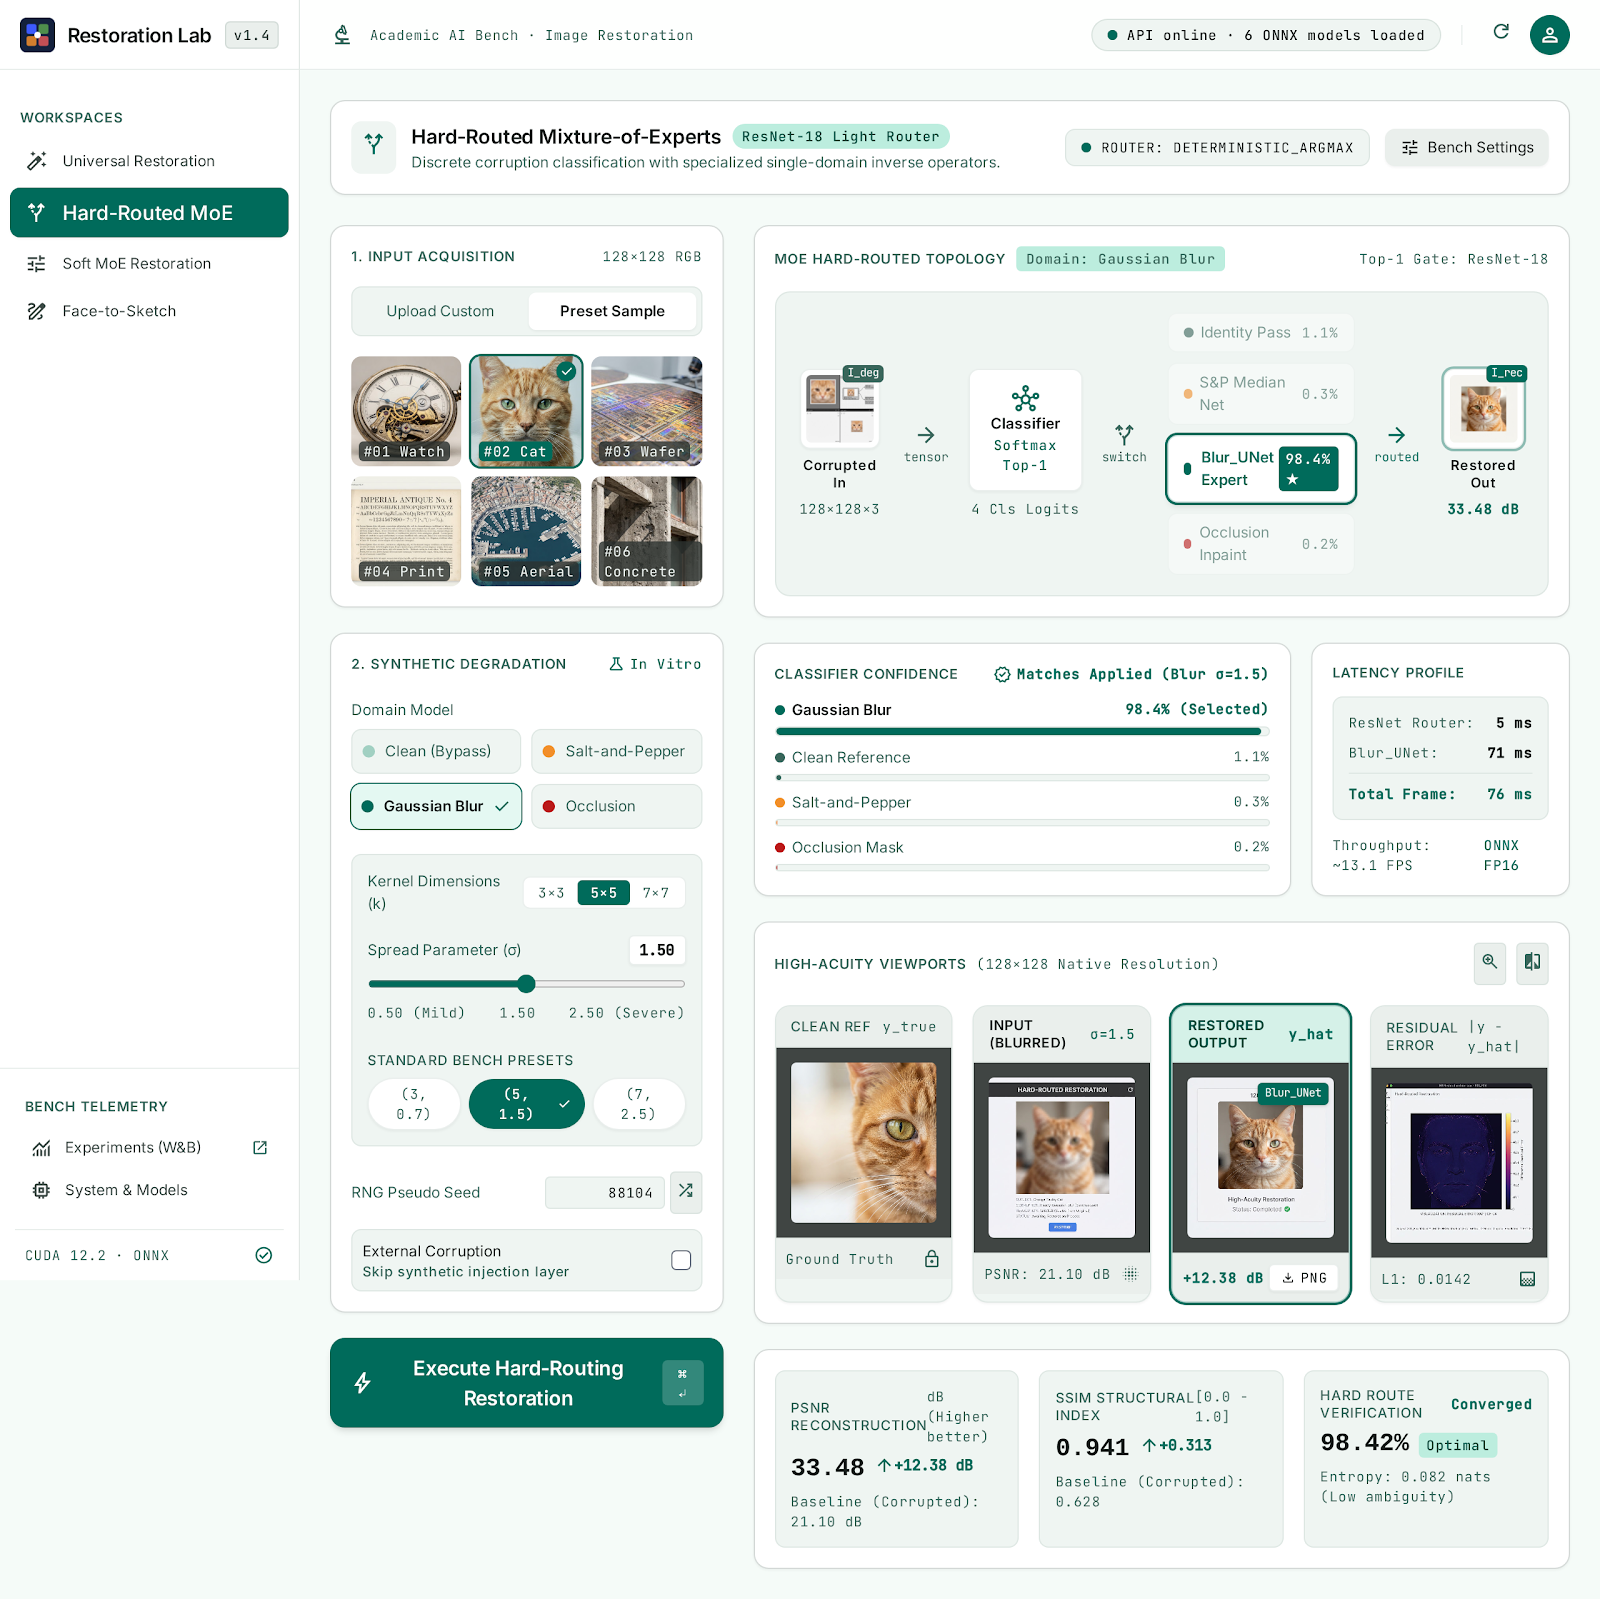
\includegraphics[width=\columnwidth]{hard-routed-restoration/screen.png}
    \caption{Google Stitch design for Hard-Routed Restoration workspace.}
    \label{fig:stitch_hard}
\end{figure}

\begin{figure}[h]
    \centering
    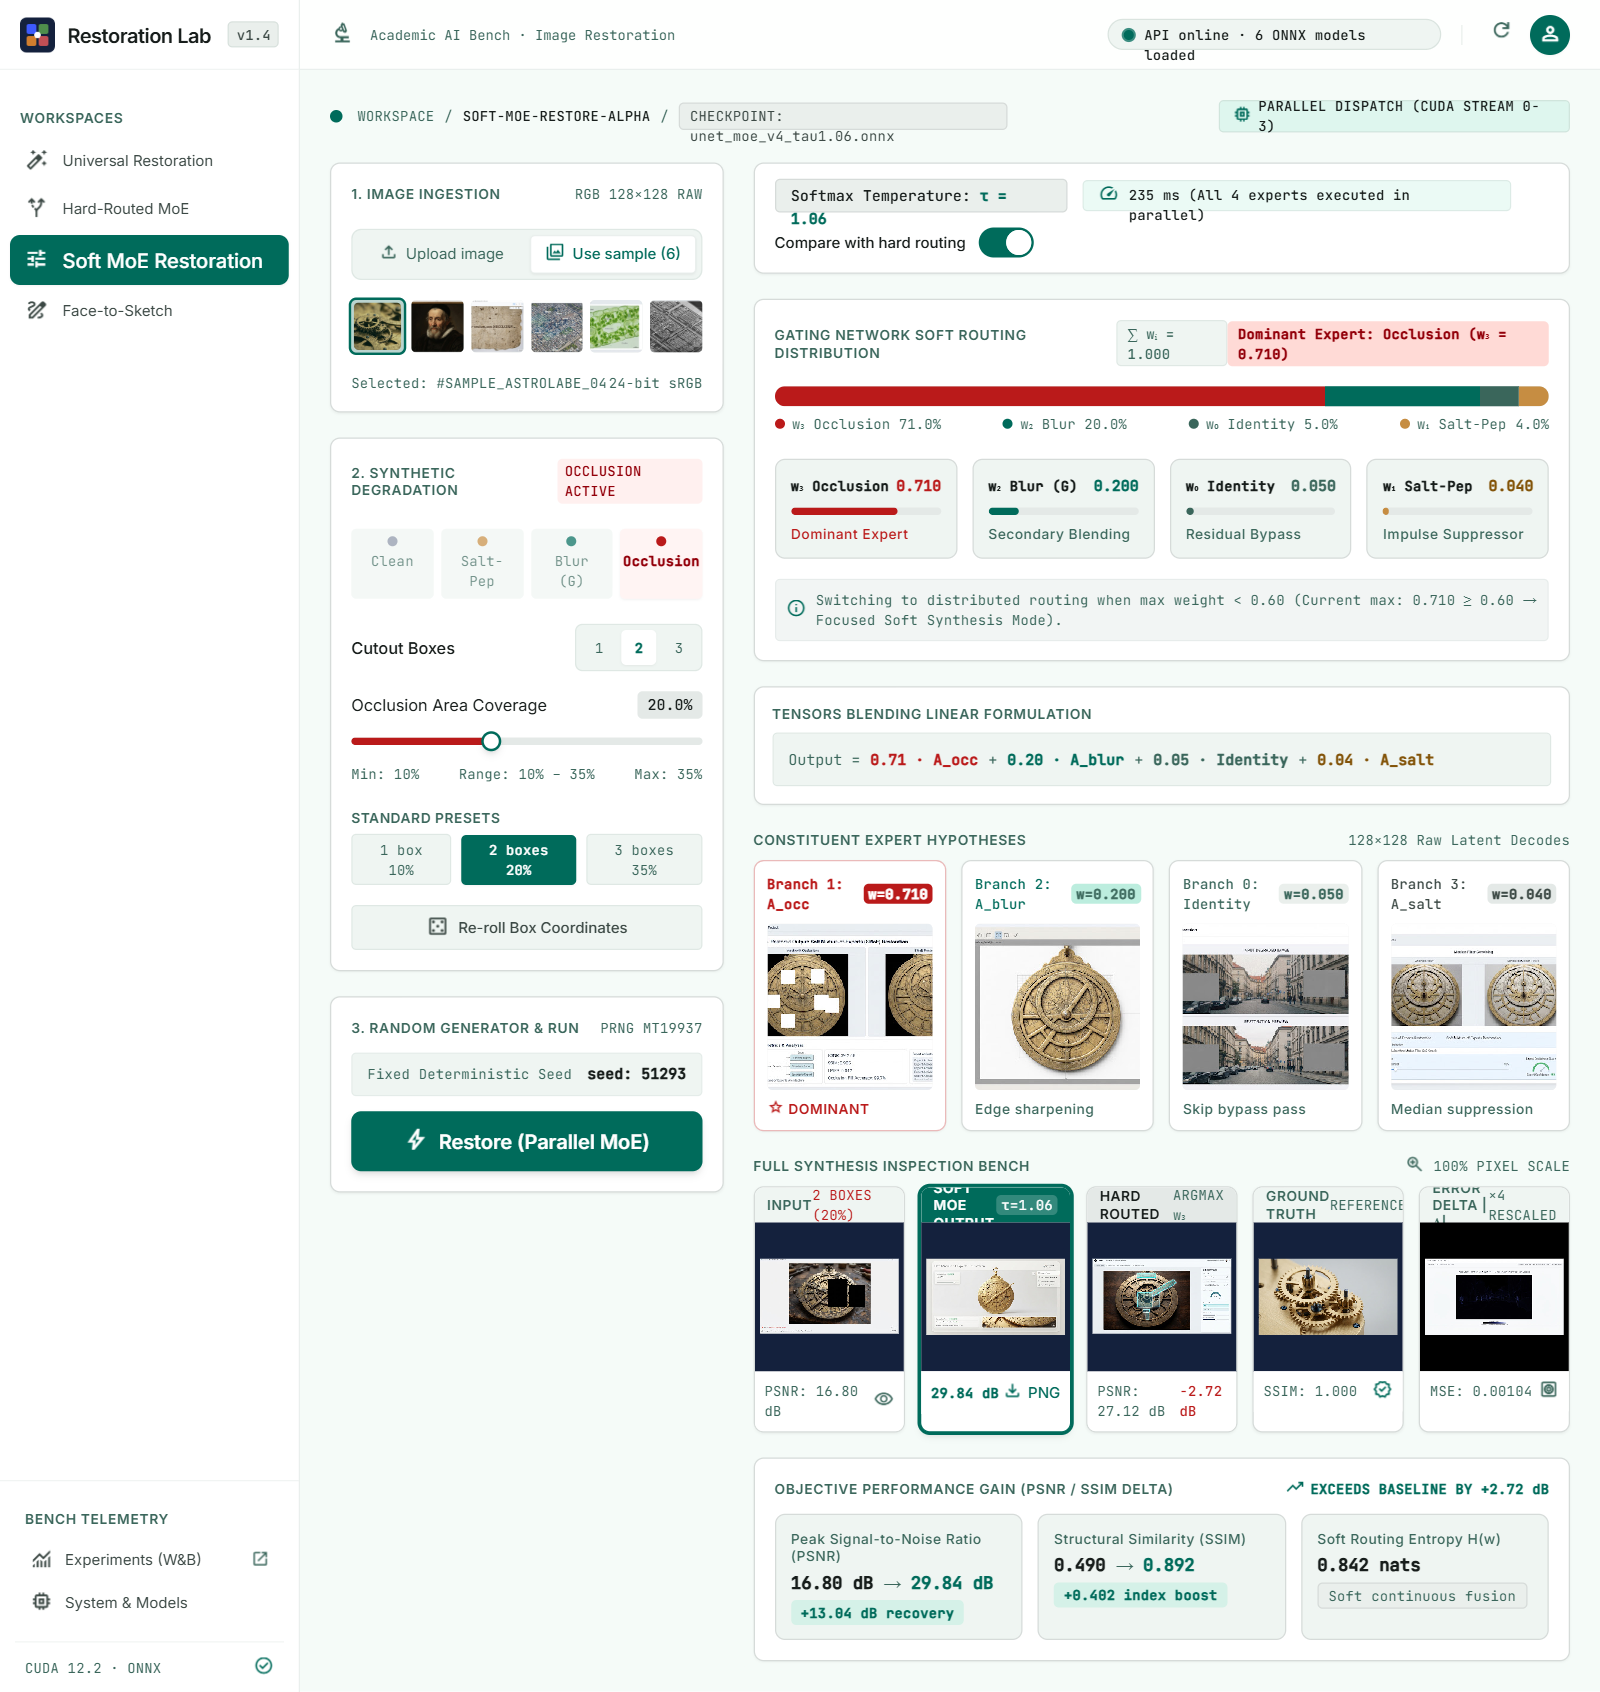
\includegraphics[width=\columnwidth]{soft-mixture-of-experts-restoratoin/screen.png}
    \caption{Google Stitch design for Soft MoE workspace.}
    \label{fig:stitch_soft}
\end{figure}

\begin{figure}[h]
    \centering
    
\includegraphics[width=\columnwidth]{face-to-sketch/screen.png}
    \caption{Google Stitch design for Face-to-Sketch workspace.}
    \label{fig:stitch_sketch}
\end{figure}

\subsection{Frontend}

Built with React~19, Tailwind~CSS~4, and Vite~8. The application uses React Router for navigation between four workspace pages. Components include:
\begin{itemize}
    \item \texttt{ImageSource}: upload/drag-and-drop with automatic $128 \times 128$ resizing, or sample selection from bundled images.
    \item \texttt{CorruptionControls}: corruption type and severity selection.
    \item \texttt{ImageViewport}: side-by-side display of input and output with zoom.
    \item \texttt{MetricTile}: inference time, PSNR, routing weights display.
\end{itemize}

\subsection{Backend}

Built with FastAPI and ONNX Runtime. The backend loads all ONNX models at startup, validates uploads, preprocesses images to $128 \times 128$ RGB $[0, 1]$ tensors, runs inference, and returns base64-encoded results with metadata (routing weights, inference time, corruption parameters).

\subsection{Deployment}

The complete application runs via Docker Compose with two services:
\begin{itemize}
    \item \textbf{Backend}: Python 3.11 slim image, ONNX Runtime CPU, models mounted read-only.
    \item \textbf{Frontend}: Node.js build stage + Nginx for static serving with API reverse proxy.
\end{itemize}

Single-command startup: \texttt{docker compose up --build}.

% ============================================================================
\section{Experiment Tracking}

All training experiments were tracked with Weights~\&~Biases. Logged metrics include per-epoch training/validation loss, PSNR, SSIM, per-corruption breakdowns, learning rate schedules, and sample reconstruction grids. Optuna trial parameters and scores were also logged.

The full W\&B project dashboard is available at: \url{https://forge.coreweave.com/wandb/umairishuman-national-university-of-computer-and-emergin/genai-assignment1}. Local run logs are also stored in \texttt{app/AI/wandb/} for offline access.

% ============================================================================
\section{Limitations}

\begin{itemize}
    \item \textbf{Resolution}: all models operate at $128 \times 128$, which limits fine detail preservation. Higher-resolution training would improve results but requires more compute.
    \item \textbf{Compound corruptions}: the system is trained on single corruptions only. Compound degradations (e.g., blur + occlusion) are handled via the soft MoE's weighted blending but not explicitly trained for.
    \item \textbf{Task~4 data imbalance}: Style~3 has very few samples (46 test images), making metrics noisy and limiting generalization.
    \item \textbf{Gaussian blur PSNR}: the universal model slightly reduces PSNR on mildly blurred images, though perceptual quality improves.
\end{itemize}

% ============================================================================
\section{Conclusion}

This work demonstrates three progressively sophisticated image restoration architectures. The universal autoencoder provides a strong single-model baseline (24.72~dB). Hard routing with specialist experts slightly improves quality (24.86~dB) through corruption-specific training. The soft mixture-of-experts achieves the best results (25.59~dB) by learning to blend expert outputs with data-driven routing weights. The conditional GAN successfully generates style-controlled sketches with an FID of 33.29.

All models are exported to ONNX and deployed in a cohesive browser-based application with Docker containerization, demonstrating the full pipeline from research and training to production deployment.

% ============================================================================
\section*{AI-Use Appendix}

\begin{itemize}
    \item \textbf{Claude Code (Anthropic)}: used for coding assistance (frontend components, backend API endpoints, Docker configuration), debugging, and documentation generation. All generated code was reviewed, tested, and modified as needed.
    \item \textbf{Google Stitch}: used for UI mockup design.
    \item \textbf{GitHub Copilot}: used for code autocompletion during training script development. Suggestions were reviewed before acceptance.
\end{itemize}

All AI-generated outputs were verified through testing (unit tests, integration tests, manual testing with the application), and the author understands the complete implementation.

% ============================================================================
\begin{thebibliography}{9}
\bibitem{vincent2008} P.~Vincent, H.~Larochelle, Y.~Bengio, and P.-A.~Manzagol, ``Extracting and composing robust features with denoising autoencoders,'' in \emph{ICML}, 2008.
\bibitem{wang2004ssim} Z.~Wang, A.~C.~Bovik, H.~R.~Sheikh, and E.~P.~Simoncelli, ``Image quality assessment: from error visibility to structural similarity,'' \emph{IEEE Trans.\ Image Processing}, vol.~13, no.~4, pp.~600--612, 2004.
\bibitem{shazeer2017} N.~Shazeer, A.~Mirhoseini, K.~Malinowski, et al., ``Outrageously large neural networks: The sparsely-gated mixture-of-experts layer,'' in \emph{ICLR}, 2017.
\bibitem{isola2017} P.~Isola, J.-Y.~Zhu, T.~Zhou, and A.~A.~Efros, ``Image-to-image translation with conditional adversarial networks,'' in \emph{CVPR}, 2017.
\bibitem{dumoulin2017} V.~Dumoulin, J.~Shlens, and M.~Kudlur, ``A learned representation for artistic style,'' in \emph{ICLR}, 2017.
\end{thebibliography}

\end{document}
